\documentclass{report}
\usepackage[a4paper, total={7.5in, 10in}]{geometry}
\usepackage[fleqn]{amsmath}
\usepackage{amssymb}
\usepackage{amsthm}
\usepackage{enumitem}
\usepackage[]{mdframed}
\usepackage{multicol}
\usepackage{thmtools}
\usepackage{graphicx}
\usepackage{tikz}
\usepackage{tipa}
\usepackage{array, makecell, cellspace}
\setlength{\cellspacetoplimit}{13.2ex}
\setlength{\cellspacebottomlimit}{13.2ex}

\usepackage{ifxetex}

\ifxetex
      \usepackage{substitutefont}
      \substitutefont{T3}{\rmdefault}{cmr}
\fi

\usepackage{fontspec}
\setmainfont[Mapping=tex-text]{Georgia}

\title{Praktis 2\\Differentiation}
\author{Melvin Chia}

\newcommand{\sol}[1]{

      \noindent \textbf{Sol.}
}
\newcommand{\prooff}[1]{

      \noindent \textbf{Proof.}
}

\newcommand{\arc}[1]{{%
                  \setbox9=\hbox{#1}%
                  \ooalign{\resizebox{\wd9}{\height}{\texttoptiebar{\phantom{A}}}\cr#1}}}

\def\eos{\quad\hbox{\rlap{\hbox{\vrule depth 1.5pt height 2.6mm width 0.2mm \hskip 1mm \vrule height 2.6mm width 0.2mm}}{\vbox{\hrule height 0.2mm width 1.4mm \vskip 2.8mm \hrule depth 1.5pt height -0.35mm width 1.2mm}}}}

\counterwithout{equation}{chapter}
\setlength{\columnseprule}{1pt}
\setlength{\columnsep}{24pt}
\hfuzz=100pt
\setcounter{chapter}{2}

\mdfdefinestyle{MyFrame}{%
      linecolor=black,
      linewidth=1pt,
      roundcorner=20pt,
      innertopmargin=12pt, innerbottommargin=12pt, innerrightmargin=12pt,
      innerleftmargin=12pt, leftmargin = 4pt, rightmargin = 4pt
      %backgroundcolor=gray!50!white}
}

\begin{document}
\maketitle

\begin{multicols*}{2}
      \noindent\Large{\underline{\textbf{Praktis Formatif}}}
      \normalsize
      \section{Limit and its Relation to Differentiation}
      \begin{enumerate}
            \item Find the value of each of the following.
                  \begin{enumerate}
                        \item $\lim\limits_{x\to1}(x-1)$
                              \sol{}
                              \begin{flalign*}
                                    \lim\limits_{x\to1}(x-1) & = 1 - 1  \\
                                                             & = 0 \eos
                              \end{flalign*}

                        \item $\lim\limits_{x\to1}{\dfrac{x^{2}-2}{x}}$
                              \sol{}
                              \begin{flalign*}
                                    \lim\limits_{x\to1}{\dfrac{x^{2}-2}{x}} & = \dfrac{1^{2}-2}{1} \\
                                                                            & = \dfrac{-1}{1}      \\
                                                                            & = -1 \eos
                              \end{flalign*}

                        \item $\lim\limits_{x\to0}{\dfrac{2x-5}{x+3}}$
                              \sol{}
                              \begin{flalign*}
                                    \lim\limits_{x\to0}{\dfrac{2x-5}{x+3}} & = \dfrac{2(0)-5}{0+3} \\
                                                                           & = \dfrac{-5}{3}       \\
                                                                           & = -\dfrac{5}{3} \eos
                              \end{flalign*}

                        \item $\lim\limits_{x\rightarrow a}(x-a)$
                              \sol{}
                              \begin{flalign*}
                                    \lim\limits_{x\rightarrow a}(x-a) & = a - a  \\
                                                                      & = 0 \eos
                              \end{flalign*}
                  \end{enumerate}
            \item Calculate the value for each of the following.
                  \begin{enumerate}
                        \item $\lim\limits_{x\to0}{\dfrac{2x^{2}-5x}{x}}$
                              \sol{}
                              \begin{flalign*}
                                    \lim\limits_{x\to0}{\dfrac{2x^{2}-5x}{x}} & = \lim\limits_{x\to0}{\dfrac{x(2x-5)}{x}} \\
                                                                              & = \lim\limits_{x\to0}{(2x-5)}             \\
                                                                              & = 2(0) - 5                                \\
                                                                              & = -5 \eos
                              \end{flalign*}

                        \item $\lim\limits_{x\to2}{\dfrac{x^{2}-4}{x-2}}$
                              \sol{}
                              \begin{flalign*}
                                    \lim\limits_{x\to2}{\dfrac{x^{2}-4}{x-2}} & = \lim\limits_{x\to2}{\dfrac{(x-2)(x+2)}{x-2}} \\
                                                                              & = \lim\limits_{x\to2}{(x+2)}                   \\
                                                                              & = 2 + 2                                        \\
                                                                              & = 4 \eos
                              \end{flalign*}

                        \item $\lim\limits_{x\to5}{\dfrac{x^{2}+4x-45}{x-5}}$
                              \sol{}
                              \begin{flalign*}
                                    \lim\limits_{x\to5}{\dfrac{x^{2}+4x-45}{x-5}} & = \lim\limits_{x\to5}{\dfrac{(x-5)(x+9)}{x-5}} \\
                                                                                  & = \lim\limits_{x\to5}{(x+9)}                   \\
                                                                                  & = 5 + 9                                        \\
                                                                                  & = 14 \eos
                              \end{flalign*}
                        \item $\lim\limits_{x\to1}{\dfrac{\log_{\mathrm{10}}x^{2}}{\log_{\mathrm{10}}x}}$
                              \sol{}
                              \begin{flalign*}
                                    \lim\limits_{x\to1}{\dfrac{\log_{\mathrm{10}}x^{2}}{\log_{\mathrm{10}}x}} & = \lim\limits_{x\to1}{\dfrac{\log_{\mathrm{10}}x^{2}}{\log_{\mathrm{10}}x}} \\
                                                                                                              & = \lim\limits_{x\to1}{\dfrac{2\log_{\mathrm{10}}x}{\log_{\mathrm{10}}x}}    \\
                                                                                                              & = \lim\limits_{x\to1}{2}                                                    \\
                                                                                                              & = 2 \eos
                              \end{flalign*}
                  \end{enumerate}
            \item Find the value for each of the following.
                  \begin{enumerate}
                        \item $\lim\limits_{x\to9}{\dfrac{x-9}{\sqrt{x}-3}}$
                              \sol{}
                              \begin{flalign*}
                                    \lim\limits_{x\to9}{\dfrac{x-9}{\sqrt{x}-3}} & = \lim\limits_{x\to9}{\dfrac{(x-9)'}{(\sqrt{x}-3)'}}   \\
                                                                                 & = \lim\limits_{x\to9}{\dfrac{1}{\dfrac{1}{2\sqrt{x}}}} \\
                                                                                 & = \lim\limits_{x\to9}{(2\sqrt{x})}                     \\
                                                                                 & = 2\sqrt{9}                                            \\
                                                                                 & = 2(3)                                                 \\
                                                                                 & = 6 \eos
                              \end{flalign*}

                        \item $\lim\limits_{x\to-1}{\dfrac{x+1}{\sqrt{x+5}-2}}$
                              \sol{}
                              \begin{flalign*}
                                    \lim\limits_{x\to-1}{\dfrac{x+1}{\sqrt{x+5}-2}} & = \lim\limits_{x\to-1}{\dfrac{(x+1)'}{(\sqrt{x+5}-2)'}}   \\
                                                                                    & = \lim\limits_{x\to-1}{\dfrac{1}{\dfrac{1}{2\sqrt{x+5}}}} \\
                                                                                    & = \lim\limits_{x\to-1}{(2\sqrt{x+5})}                     \\
                                                                                    & = 2\sqrt{-1+5}                                            \\
                                                                                    & = 2\sqrt{4}                                               \\
                                                                                    & = 2(2)                                                    \\
                                                                                    & = 4 \eos
                              \end{flalign*}

                        \item $\lim\limits_{x\to9}{\dfrac{\sqrt{x+7}-4}{x-9}}$
                              \sol{}
                              \begin{flalign*}
                                    \lim\limits_{x\to9}{\dfrac{\sqrt{x+7}-4}{x-9}} & = \lim\limits_{x\to9}{\dfrac{(\sqrt{x+7}-4)'}{(x-9)'}} \\
                                                                                   & = \lim\limits_{x\to9}{\dfrac{1}{2\sqrt{x+7}}}          \\
                                                                                   & = \dfrac{1}{2\sqrt{9+7}}                               \\
                                                                                   & = \dfrac{1}{8}                                         \\
                              \end{flalign*}
                        \item $\lim\limits_{x\to2}{\dfrac{\sqrt{6-x}-2}{3-{\sqrt{11-x}}}}$
                              \sol{}
                              \begin{flalign*}
                                    \lim\limits_{x\to2}{\dfrac{\sqrt{6-x}-2}{3-{\sqrt{11-x}}}} & = \lim\limits_{x\to2}{\dfrac{(\sqrt{6-x}-2)'}{(3-{\sqrt{11-x}})'}}              \\
                                                                                               & = \lim\limits_{x\to2}{\dfrac{\dfrac{1}{2\sqrt{6-x}}}{\dfrac{1}{-2\sqrt{11-x}}}} \\
                                                                                               & = \lim\limits_{x\to2}{\dfrac{-2\sqrt{11-x}}{2\sqrt{6-x}}}                       \\
                                                                                               & = \lim\limits_{x\to2}{\dfrac{-\sqrt{11-x}}{\sqrt{6-x}}}                         \\
                                                                                               & = -\dfrac{\sqrt{11-2}}{\sqrt{6-2}}                                              \\
                                                                                               & = -\dfrac{3}{2} \eos
                              \end{flalign*}
                  \end{enumerate}
            \item The following diagram shows part of a graph $y = f(x)$.
                  \begin{center}
                        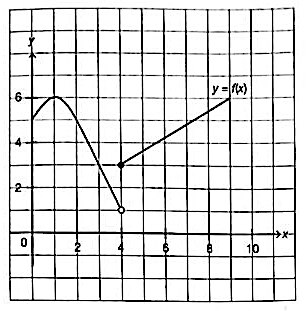
\includegraphics[width=0.4\textwidth]{./images/q4.jpeg}
                  \end{center}
                  Based on this graph, find
                  \begin{enumerate}
                        \item $f(4)$
                              \sol{}
                              \begin{flalign*}
                                    f(4) & = 3
                              \end{flalign*}

                        \item $\lim\limits_{x\to4}{f(x)}$ and explain your answer.
                              \sol{}
                              \begin{flalign*}
                                    \lim_{x\to4^-}{f(x)} & \neq 4 \\
                                    \lim_{x\to4^+}{f(x)} & = 4    \\
                              \end{flalign*}
                              Since the left limit and right limit are different, $f(4)$ does not exist.

                        \item $\lim\limits_{x\to1}{f(x)}$
                              \sol{}
                              \begin{flalign*}
                                    \lim_{x\to1}{f(x)} & = 6 \\
                              \end{flalign*}
                  \end{enumerate}

            \item Find $\dfrac{dy}{dx}$ by using the first principle.
                  \begin{enumerate}
                        \item $y = 3x + 5$
                              \sol{}
                              \begin{flalign*}
                                    y                          & = 3x + 5                                                              & (1) \\
                                    y + \delta y               & = 3(x + \delta x) + 5                                                       \\
                                    y + \delta y               & = 3x + 3\delta x + 5                                                  & (2) \\
                                    (2) - (1):                 &                                                                             \\
                                    \delta y                   & = 3\delta x                                                                 \\
                                    \dfrac{\delta y}{\delta x} & = 3                                                                         \\
                                    \therefore\ \dfrac{dy}{dx} & = \lim\limits_{\delta x\to0}{\left(\dfrac{\delta y}{\delta x}\right)}       \\
                                                               & = \lim\limits_{\delta x\to0}{3}                                             \\
                                                               & = 3 \eos
                              \end{flalign*}

                        \item $y = x^2 - 7$
                              \sol{}
                              \begin{flalign*}
                                    y                          & = x^2 - 7                                                             & (1) \\
                                    y + \delta y               & = (x + \delta x)^2 - 7                                                      \\
                                    y + \delta y               & = x^2 + 2x\delta x + {(\delta x)}^2 - 7                               & (2) \\
                                    (2) - (1):                 &                                                                             \\
                                    \delta y                   & = 2x\delta x + {(\delta x)}^2                                               \\
                                    \dfrac{\delta y}{\delta x} & = 2x + 2\delta x                                                            \\
                                    \therefore\ \dfrac{dy}{dx} & = \lim\limits_{\delta x\to0}{\left(\dfrac{\delta y}{\delta x}\right)}       \\
                                                               & = \lim\limits_{\delta x\to0}{(2x + 2\delta x)}                              \\
                                                               & = 2x \eos
                              \end{flalign*}

                        \item $y = x^2 + 2x + 1$
                              \sol{}
                              \begin{flalign*}
                                    y                          & = x^2 + 2x + 1                                                        & (1) \\
                                    y + \delta y               & = (x + \delta x)^2 + 2(x + \delta x) + 1                                    \\
                                    y + \delta y               & = x^2 + 2x\delta x + {(\delta x)}^2 + 2x + 2\delta x                        \\
                                                               & \ \ \ \ + 1                                                           & (2) \\
                                    (2) - (1):                 &                                                                             \\
                                    \delta y                   & = 2x\delta x + {(\delta x)}^2 + 2\delta x                                   \\
                                    \dfrac{\delta y}{\delta x} & = 2x + \delta x + 2                                                         \\
                                    \therefore\ \dfrac{dy}{dx} & = \lim\limits_{\delta x\to0}{\left(\dfrac{\delta y}{\delta x}\right)}       \\
                                                               & = \lim\limits_{\delta x\to0}{(2x + \delta x + 2)}                           \\
                                                               & = 2x + 2 \eos
                              \end{flalign*}

                        \item $y = -x^3 + 9$
                              \sol{}
                              \begin{flalign*}
                                    y                          & = -x^3 + 9                                                                     & (1) \\
                                    y + \delta y               & = -(x + \delta x)^3 + 9                                                              \\
                                    y + \delta y               & = -x^3 - 3x^2\delta x - 3x{(\delta x)}^2 - \delta x^3                                \\
                                                               & \ \ \ \ + 9                                                                    & (2) \\
                                    (2) - (1):                 &                                                                                      \\
                                    \delta y                   & = -3x^2\delta x - 3x{(\delta x)}^2 - \delta x^3                                      \\
                                    \dfrac{\delta y}{\delta x} & = -3x^2 - 3x\delta x - {(\delta x)}^2                                                \\
                                    \therefore\ \dfrac{dy}{dx} & = \lim\limits_{\delta x\to0}{\left(\dfrac{\delta y}{\delta x}\right)}                \\
                                                               & = \lim\limits_{\delta x\to0}{\left[-3x^2 - 3x\delta x - {(\delta x)}^2\right]}       \\
                                                               & = -3x^2 \eos
                              \end{flalign*}

                        \item $y = 2 - \dfrac{3}{x}$
                              \sol{}
                              \begin{flalign*}
                                    y                          & = 2 - 3x^{-1}                                                         & (1) \\
                                    y + \delta y               & = 2 - 3{(x + \delta x)}^{-1}                                          & (2) \\
                                    (2) - (1):                 &                                                                             \\
                                    \delta y                   & = -3{(x + \delta x)}^{-1} + 3x^{-1}                                         \\
                                                               & = -\frac{3}{x + \delta x} + \frac{3}{x}                                     \\
                                                               & = \frac{-3x + 3x + 3\delta x}{x(x + \delta x)}                              \\
                                                               & = \frac{3\delta x}{x^2 + x\delta x}                                         \\
                                    \dfrac{\delta y}{\delta x} & = \frac{3}{x^2 + x\delta x}                                                 \\
                                    \therefore\ \dfrac{dy}{dx} & = \lim\limits_{\delta x\to0}{\left(\dfrac{\delta y}{\delta x}\right)}       \\
                                                               & = \lim\limits_{\delta x\to0}{\left(\frac{3}{x^2 + x\delta x}\right)}        \\
                                                               & = \frac{3}{x^2} \eos
                              \end{flalign*}
                  \end{enumerate}

            \item Given a curve $y = x^2 - ax + b$
                  \begin{enumerate}
                        \item By using the first principle, find the gradient function to the curve. \sol{}
                              \begin{flalign*}
                                    y                          & = x^2 - ax + b                                                        & (1) \\
                                    y + \delta y               & = (x + \delta x)^2 - a(x + \delta x) + b                                    \\
                                    y + \delta y               & = x^2 + 2x\delta x + {(\delta x)}^2 - ax - a\delta x                        \\
                                                               & \ \ \ \ + b                                                           & (2) \\
                                    (2) - (1):                 &                                                                             \\
                                    \delta y                   & = 2x\delta x + {(\delta x)}^2 - a\delta x                                   \\
                                    \dfrac{\delta y}{\delta x} & = 2x + \delta x - a                                                         \\
                                    \therefore\ \dfrac{dy}{dx} & = \lim\limits_{\delta x\to0}{\left(\dfrac{\delta y}{\delta x}\right)}       \\
                                                               & = \lim\limits_{\delta x\to0}{(2x + \delta x - a)}                           \\
                                                               & = 2x - a \eos
                              \end{flalign*}

                        \item Given that the value of gradient of the curve at $(2, -3)$ is $2$, find the
                              value of $a$ and $b$. \sol{}
                              \begin{flalign*}
                                    \dfrac{dy}{dx} & = 2x - a             \\
                                    2              & = 2(2) - a           \\
                                    \therefore\ a  & = 2 \eos             \\
                                    \\
                                    y              & = x^2 - 2x + b       \\
                                    -3             & = {(2)}^2 - 2(2) + b \\
                                    -3             & = 4 - 4 + b          \\
                                    \therefore\ b  & = -3 \eos
                              \end{flalign*}
                  \end{enumerate}
      \end{enumerate}

      \section{The First Derivative}

      \begin{enumerate}
            \setcounter{enumi}{6}
            \item Find the first derivative for each of the following functions.
                  \begin{enumerate}
                        \item $y = 6x^2$
                              \sol{}
                              \begin{flalign*}
                                    \dfrac{dy}{dx} & = 12x \eos
                              \end{flalign*}

                        \item $y = -x^4$
                              \sol{}
                              \begin{flalign*}
                                    \dfrac{dy}{dx} & = -4x^3 \eos
                              \end{flalign*}

                        \item $y = \sqrt[3]{x^4}$
                              \sol{}
                              \begin{flalign*}
                                    y              & = x^{\frac{4}{3}}                \\
                                    \dfrac{dy}{dx} & = \frac{4}{3}x^{\frac{4}{3} - 1} \\
                                                   & = \frac{4}{3}\sqrt[3]{x} \eos
                              \end{flalign*}

                        \item $y = -\frac{2}{x^2}$
                              \sol{}
                              \begin{flalign*}
                                    y              & = -2x^{-2}                \\
                                    \dfrac{dy}{dx} & = -2\left(-2x^{-3}\right) \\
                                                   & = 4x^{-3}                 \\
                                                   & = \frac{4}{x^3} \eos
                              \end{flalign*}
                  \end{enumerate}

            \item Find each of the following.
                  \begin{enumerate}
                        \item ${\dfrac{d}{d x}}\Big(2x^{2}+3x-9{\Big)}$
                              \sol{}
                              \begin{flalign*}
                                    \dfrac{d}{d x}\Big(2x^{2}+3x-9{\Big)} & = 4x + 3 \eos
                              \end{flalign*}
                        \item ${\dfrac{d}{d x}}\left(x^{2}+{\dfrac{2}{x}}\right)$
                              \sol{}
                              \begin{flalign*}
                                    \dfrac{d}{d x}\left(x^{2}+{\dfrac{2}{x}}\right) & = \dfrac{d}{dx}\left(x^2 + 2x^{-1}\right) \\
                                                                                    & = 2x -2x^{-2}                             \\
                                                                                    & = 2x - \dfrac{2}{x^2}\eos
                              \end{flalign*}
                        \item ${\dfrac{d}{d x}}\left(5x^{3}+2x^{2}+4x-7-{\dfrac{1}{x}}+{\dfrac{3}{x^{2}}}\right)$
                              \sol{}
                              \begin{flalign*}
                                     & \dfrac{d}{d x}\left(5x^{3}+2x^{2}+4x-7-{\dfrac{1}{x}}+{\dfrac{3}{x^{2}}}\right) \\
                                     & = \dfrac{d}{d x}\left(5x^{3}+2x^{2}+4x-7-x^{-1}+3x^{-2}\right)                  \\
                                     & = 15x^2 + 4x + 4 + x^{-2} - 6x^{-3}                                             \\
                                     & = 15x^2 + 4x + 4 + \dfrac{1}{x^2} - \dfrac{6}{x^3}     \eos
                              \end{flalign*}
                  \end{enumerate}

            \item Differentiate each of the following functions with respect to x.
                  \begin{enumerate}
                        \item $f(x)=x\left({\dfrac{1}{2}}x^{4}-x^{2}-5x\right)$
                              \sol{}
                              \begin{flalign*}
                                    f(x)         & = \frac{1}{2}x^5 - x^3 - 5x^2      \\
                                    \frac{d}{dx} & = \frac{5}{2}x^4 - 3x^2 - 10x \eos
                              \end{flalign*}

                        \item $f(x)=(x^{2}-5)(x+3)$
                              \sol{}
                              \begin{flalign*}
                                    f(x)         & = x^3 + 3x^2 - 5x - 15 \\
                                    \frac{d}{dx} & = 3x^2 + 6x - 5 \eos
                              \end{flalign*}
                        \item $f(x)={\dfrac{(x^{3}-x+4)}{x}}$
                              \sol{}
                              \begin{flalign*}
                                    f(x)         & = \frac{x^2}{x} - 1 + \frac{4}{x} \\
                                                 & = x^2 - 1 + 4x^{-1}               \\
                                    \frac{d}{dx} & = 2x - 4x^{-2}                    \\
                                                 & = 2x - \frac{4}{x^2} \eos
                              \end{flalign*}
                        \item $f(x)={\frac{(x^{2}-x-2)}{(x-2)}}$
                              \sol{}
                              \begin{flalign*}
                                    f(x)         & = \frac{(x-2)(x+1)}{x-2} \\
                                                 & = x+1                    \\
                                    \frac{d}{dx} & = 1 \eos
                              \end{flalign*}
                  \end{enumerate}

            \item Find $f'(x)$ for each of the following functions.
                  \begin{enumerate}
                        \item $f(x)={(3x-5)}^{4}$
                              \sol{}
                              \begin{flalign*}
                                    f'(x) & = 4{(3x-5)}^3 \cdot \frac{d}{dx}(3x-5) \\
                                          & = 4{(3x-5)}^3 \cdot 3                  \\
                                          & = 12{(3x-5)}^2 \eos
                              \end{flalign*}

                        \item $f(x)=5{(x^{3}+4x)}^{3}$
                              \sol{}
                              \begin{flalign*}
                                    f'(x) & = 5{(x^{3}+4x)}^3 \cdot \frac{d}{dx}(x^3+4x)  \\
                                          & = 5{(x^{3}+4x)}^3 \cdot \left(3x^2 + 4\right) \\
                                          & = 15\left(3x^2 + 4\right){(x^{3}+4x)}^2 \eos
                              \end{flalign*}

                        \item $f(x)={\dfrac{2}{{(5x^{2}-3x)}^{10}}}$
                              \sol{}
                              \begin{flalign*}
                                    f(x) & = \frac{-20\cdot \dfrac{d}{dx}{(5x^2 - 3x)}}{{(5x^2-3x)}^{11}} \\
                                         & = \frac{-20(10x - 3)}{{(5x^2-3x)}^{11}}                        \\
                              \end{flalign*}
                  \end{enumerate}

            \item Find the first derivative for each of the following functions by using the
                  product rule.
                  \begin{enumerate}
                        \item $y=6x^{2}{(x+5x^{2})}^{3}$
                              \sol{}
                              \begin{flalign*}
                                    y             & = 6x^2{[x(1+5x)]}^3                                       \\
                                                  & = 6x^2(x^3){(1+5x)}^3                                     \\
                                                  & = 6x^5{(1+5x)}^3                                          \\
                                    \\
                                    \frac{dy}{dx} & = 6x^5\frac{d}{dx}{(1+5x)}^3 + {(1+5x)}^3\frac{d}{dx}6x^5 \\
                                                  & = 6x^5\cdot5\cdot 3{(1+5x)}^2 + 30x^4{(1+5x)}^3           \\
                                                  & = 90x^5\cdot{(1+5x)}^2 + 30x^4{(1+5x)}^3                  \\
                                                  & = 30x^4{(1+5x)}^2(1+5x + 3x)                              \\
                                                  & = 30x^4{(5x+1)}^2(8x+1)                                   \\
                              \end{flalign*}

                        \item $y=x{(7x+3)}^{5}$
                              \sol{}
                              \begin{flalign*}
                                    \frac{dy}{dx} & = x\frac{d}{dx}(7x+3)^5 + (7x+3)^5\frac{d}{dx}x \\
                                                  & = x\cdot5{(7x+3)}^4\cdot7 + {(7x+3)}^5\cdot1    \\
                                                  & = 35x{(7x+3)}^4 + {(7x+3)}^5                    \\
                                                  & = {(7x+3)}^4(35x + 7x + 3)                      \\
                                                  & = {(7x+3)}^4(42x + 3) \eos
                              \end{flalign*}
                        \item $y={(4x^{2}-3x)(1-2x^{2})}^{10}$
                              \sol{}
                              \begin{flalign*}
                                    \frac{dy}{dx} & = (4x^2-3x)\frac{d}{dx}{(1-2x^2)}^{10} + (1-2x^2)^{10}   \\
                                                  & \ \ \ \ \frac{d}{dx}(4x^2-3x)                          & \\
                                                  & = (4x^2-3x)\cdot10{(1-2x^2)}^9\cdot(-4x) + (1            \\
                                                  & \ \ \ \ -2x^2)^{10}(8x - 3)                              \\
                                                  & = {(1-2x^2)}^{9}[(-40x)(4x^2-3x) + (1-2x^2)              \\
                                                  & \ \ \ \ (8x-3)]                                          \\
                                                  & = {(1-2x^2)}^{9}[-160x^3 + 120x^2 + 8x - 3               \\
                                                  & \ \ \ \ -16x^3+6x^2]                                     \\
                                                  & = {(1-2x^2)}^{9}[-176x^3 + 126x^2 + 8x - 3] \eos
                              \end{flalign*}
                  \end{enumerate}

            \item Find $\dfrac{dy}{dx}$ for each of the following functions by using the quotient
                  rule.
                  \begin{enumerate}
                        \item $y={\dfrac{x-2}{2x+1}}$
                              \sol{}
                              \begin{flalign*}
                                    \frac{dy}{dx} & = \dfrac{(2x + 1)\dfrac{d}{dx}(x-2) - (x-2)\dfrac{d}{dx}(2x + 1)}{{(2x+1)}^2} & \\
                                                  & = \dfrac{2x + 1 - 2(x-2)}{{(2x+1)}^2}                                         & \\
                                                  & = \dfrac{5}{{(2x+1)}^2} \eos
                              \end{flalign*}

                        \item $y={\dfrac{x^{2}+3x-4}{x-1}}$
                              \sol{}
                              \begin{flalign*}
                                    y             & = \dfrac{(x+4)(x-1)}{x-1} \\
                                                  & = x + 4                   \\
                                    \\
                                    \frac{dy}{dx} & = 1 \eos
                              \end{flalign*}

                        \item $y={\dfrac{x^{3}}{{(2x-1)}^{2}}}$
                              \sol{}
                              \begin{flalign*}
                                    \frac{dy}{dx} & = \dfrac{{(2x-1)}^2\dfrac{d}{dx}(x^3) - (x^3)\dfrac{d}{dx}{(2x-1)}^2}{{(2x-1)}^4} & \\
                                                  & = \dfrac{{(2x-1)}^2\cdot3x^2 - x^3\cdot4(2x-1)}{{(2x-1)}^4}                       & \\
                                                  & = \dfrac{(2x-1)[3x^2(2x-1)- 4x^3]}{{(2x-1)}^4}                                    & \\
                                                  & = \dfrac{6x^3-3x^2- 4x^3}{{(2x-1)}^3}                                             & \\
                                                  & = \dfrac{2x^3-3x^2}{{(2x-1)}^3}                                                   & \\
                                                  & = \dfrac{x^2(2x-3)}{{(2x-1)}^3} \eos
                              \end{flalign*}
                  \end{enumerate}

            \item Find the gradient function to the curve $y = \sqrt{x}(4x+1)$. Hence, find the
                  value of the gradient of the curve at $x = 4$. \sol{}
                  \begin{flalign*}
                        y              & = \sqrt{x}(4x+1)                                                         \\
                                       & = 4x\sqrt{x} + \sqrt{x}                                                  \\
                                       & = 4x\cdot {x^{\frac{1}{2}}} + {x^{\frac{1}{2}}}                          \\
                                       & = 4x^{\frac{3}{2}} + x^{\frac{1}{2}}                                     \\
                        \\
                        \dfrac{dy}{dx} & = 4\left(\frac{3}{2}x^{\frac{1}{2}}\right) + \frac{1}{2}x^{-\frac{1}{2}} \\
                                       & = 6\sqrt{x} + \frac{1}{2\sqrt{x}} \eos                                   \\
                        \\
                        \text{When }   & x = 4,                                                                   \\
                        \dfrac{dy}{dx} & = 6\sqrt{4} + \frac{1}{2\sqrt{4}}                                        \\
                                       & = 12 + \frac{1}{4}                                                       \\
                                       & = \frac{49}{4} \eos
                  \end{flalign*}
            \item Given $x^2y = 5$, find $\dfrac{dy}{dx}$ when $x = 2$. \sol{}
                  \begin{flalign*}
                        x^2y           & = 5                           \\
                        y              & = \frac{5}{x^2}               \\
                                       & = 5x^{-2}                     \\
                        \\
                        \dfrac{dy}{dx} & = 5(-2x^{-3})                 \\
                                       & = -10x^{-3}                   \\
                        \\
                        \text{When }   & x = 2,                        \\
                        \dfrac{dy}{dx} & = -10(2)^{-3}                 \\
                                       & = -10\left(\frac{1}{8}\right) \\
                                       & = -\frac{5}{4} \eos
                  \end{flalign*}

            \item Given $y = 5x^m$ and $\dfrac{dy}{dx} = x^n$, find the value of $m$ and $n$.
                  \sol{}
                  \begin{flalign*}
                        \dfrac{dy}{dx} & = 5m\cdot x^{m-1} \\
                        x^n            & = 5mx^{m-1}       \\
                  \end{flalign*}
                  Comparing both sides,
                  \begin{flalign*}
                        5m              & = 1                 \\
                        m               & = \frac{1}{5} \eos  \\
                        m - 1           & = n                 \\
                        \frac{1}{5} - 1 & = n                 \\
                        n               & = -\frac{4}{5} \eos
                  \end{flalign*}

            \item Given $f(x) = ax^3 - bx^2 + 9x + 5$ where $a, b > 0$. Show that $f'(x)$ is
                  always positive for all the values of $x$ when $b^2 < 27a$. \sol{}
                  \begin{flalign*}
                        f'(x) & = 3ax^2 - 2bx + 9                                                                           \\
                              & = 3a\left(x^2 - \frac{2b}{3a}x\right) + 9                                                   \\
                              & = 3a\left[\left(x^2 - \frac{2b}{3a}x + \frac{b^2}{9a^2}\right) - \frac{b^2}{9a^2}\right] +9 \\
                              & = 3a{\left(x - \frac{b}{3a}\right)}^2 - \frac{b^2}{3a} + 9
                  \end{flalign*}
                  $f'(x)$ is always positive when $- \dfrac{b^2}{3a} + 9 > 0$.
                  \begin{flalign*}
                        -\frac{b^2}{3a} + 9 & > 0                             \\
                        \frac{b^2}{3a}      & < 9                             \\
                        b^2                 & < 27a \quad (\text{shown}) \eos
                  \end{flalign*}
            \item Given $\dfrac{d}{dx}(ax^m + bx^n) = 12x^s + 9x^t$ where $a, b > 0$.
                  \begin{enumerate}
                        \item Find $\dfrac{s}{t}$ in terms of $a$ and $b$. \sol{}
                              \begin{flalign*}
                                    \frac{d}{dx}(ax^m + bx^n) & = max^{m-1} + nbx^{n-1} \\
                                    12x^s + 9x^t              & = max^{m-1} + nbx^{n-1} \\
                              \end{flalign*}
                              Comparing both sides,
                              \begin{flalign*}
                                    ma          & = 12                                 \\
                                    m           & = \frac{12}{a}                       \\
                                    nb          & = 9                                  \\
                                    n           & = \frac{9}{b}                        \\
                                    s           & = m-1                                \\
                                                & = \frac{12}{a}-1                     \\
                                                & = \frac{12-a}{a}                     \\
                                    t           & = n-1                                \\
                                                & = \frac{9}{b}-1                      \\
                                                & = \frac{9-b}{b}                      \\
                                    \frac{s}{t} & = \frac{12-a}{a} \cdot \frac{b}{9-b} \\
                                                & = \frac{b(12-a)}{a(9-b)} \eos
                              \end{flalign*}

                        \item Find the values of $a$ and $b$ if $3s = 5t$ and $\frac{m}{n} = \frac{3}{2}$.
                              \sol{}
                              \begin{flalign*}
                                    3s                             & = 5t                                \\
                                    3\left(\frac{12 - a}{a}\right) & = 5\left(\frac{9-n}{b}\right)       \\
                                    \frac{36 - 3a}{a}              & = \frac{45 - 5b}{b}                 \\
                                    36b - 3ab                      & = 45a - 5ab                         \\
                                    45a - 36b - 2ab                & = 0                           & (1) \\
                                    \frac{m}{n}                    & = \frac{3}{2}                       \\
                                    \frac{12}{a} \cdot \frac{b}{9} & = \frac{3}{2}                       \\
                                    \frac{12b}{9a}                 & = \frac{3}{2}                       \\
                                    \frac{4b}{3a}                  & = \frac{3}{2}                       \\
                                    8b                             & = 9a                                \\
                                    a                              & = \frac{8b}{9}                & (2)
                              \end{flalign*}
                              Substituting (2) in (1),
                              \begin{flalign*}
                                    45\left(\frac{8b}{9}\right) - 36b - 2\left(\frac{8b}{9}\right)b                                     & = 0                    \\
                                    40b - 36b - \frac{16b^2}{9}                                                                         & = 0                    \\
                                    4b - \frac{16b^2}{9}                                                                                & = 0                    \\
                                    16b^2 - 36b                                                                                         & = 0                    \\
                                    b(4b - 9)                                                                                           & = 0                    \\
                                    b                                                               = 0 \quad \text{or} \quad b         & = \frac{9}{4}          \\
                                    \because\ b > 0, b                                                                           = 0 \  & \text{is not possible} \\
                                    \therefore\ b                                                                                       & = \frac{9}{4} \eos
                              \end{flalign*}
                              Substituting $b = \frac{9}{4}$ in (2),
                              \begin{flalign*}
                                    a & = \frac{8b}{9}                 \\
                                      & = \frac{8\cdot\dfrac{9}{4}}{9} \\
                                      & = \frac{18}{9}                 \\
                                      & = 2 \eos
                              \end{flalign*}
                        \item Hence, or otherwise, find the values of $m$, $n$, $s$, and $t$. \sol{}

                              Substituting $a = 2$ in $m = \dfrac{12}{a}$,
                              \begin{flalign*}
                                    m & = \dfrac{12}{a} \\
                                      & = \dfrac{12}{2} \\
                                      & = 6 \eos
                              \end{flalign*}
                              Substituting $b = \dfrac{9}{4}$ in $n = \dfrac{9}{b}$,
                              \begin{flalign*}
                                    n & = \dfrac{9}{b}            \\
                                      & = \dfrac{9}{\dfrac{9}{4}} \\
                                      & = 4 \eos
                              \end{flalign*}
                              Substituting $a = 2$ in $s = m - 1$,
                              \begin{flalign*}
                                    s & = m - 1  \\
                                      & = 6 - 1  \\
                                      & = 5 \eos
                              \end{flalign*}
                              Substituting $b = \dfrac{9}{4}$ in $t = n - 1$,
                              \begin{flalign*}
                                    t & = n - 1  \\
                                      & = 4 - 1  \\
                                      & = 3 \eos
                              \end{flalign*}
                  \end{enumerate}
      \end{enumerate}

      \section{The Second Derivative}
      \begin{enumerate}
            \setcounter{enumi}{17}
            \item Find $\dfrac{dy}{dx}$ and $\dfrac{d^2y}{dx^2}$ for each of the following.
                  \begin{enumerate}
                        \item $y = 4x^3 + 7x^{-1}$
                              \sol{}
                              \begin{flalign*}
                                    \dfrac{dy}{dx}     & = 12x^2 - 7x^{-2} \eos \\
                                    \dfrac{d^2y}{dx^2} & = 24x + 14x^{-3} \eos
                              \end{flalign*}

                        \item $y = {(2x^3-3)}^5$
                              \sol{}
                              \begin{flalign*}
                                    \dfrac{dy}{dx}     & = 5{(2x^3 - 3)}^4(6x^2)                    \\
                                                       & = 30x^2{(2x^3 - 3)}^4 \eos                 \\
                                    \dfrac{d^2y}{dx^2} & = 60x{(2x^3 - 3)}^4 + 720x^4{(2x^3 - 3)}^3 \\
                                                       & = 60x{(2x^3 - 3)}^3(2x^3 - 3 + 12x^3)      \\
                                                       & = 60x{(2x^3 - 3)}^3(14x^3 - 3) \eos
                              \end{flalign*}

                        \item $y = \dfrac{4}{3}\pi x^3$
                              \sol{}
                              \begin{flalign*}
                                    \dfrac{dy}{dx}     & = \dfrac{4}{3}\pi(3x^2) \\
                                                       & = 4\pi x^2 \eos         \\
                                    \dfrac{d^2y}{dx^2} & = \dfrac{4}{3}\pi(6x)   \\
                                                       & = 8\pi x \eos
                              \end{flalign*}
                        \item $y = \dfrac{3}{{(x^2 + 1)}^2}$
                              \sol{}
                              \begin{flalign*}
                                    \frac{dy}{dx}     & = \frac{0 - 3(2)(x^2 + 1)(2x)}{{(x^2 + 1)}^4}                     \\
                                                      & = \frac{-12x(x^2 + 1)}{{(x^2 + 1)}^4}                             \\
                                                      & = \frac{-12x}{{(x^2 + 1)}^3} \eos                                 \\
                                    \frac{d^2y}{dx^2} & = \frac{-12{(x^2 + 1)}^3 +12x(3){(x^2 + 1)}^2(2x)}{{(x^2 + 1)}^6} \\
                                                      & = \frac{-12{(x^2 + 1)}^3 + 72x^2{(x^2 + 1)}^2}{{(x^2 + 1)}^6}     \\
                                                      & = \frac{-12{(x^2 + 1)}^2(x^2 + 1 - 6x^2)}{{(x^2 + 1)}^6}          \\
                                                      & = \frac{-12(1-5x^2)}{{(x^2 + 1)}^4} \eos
                              \end{flalign*}
                  \end{enumerate}

            \item Given a curve $y = 4x^3 - 2x^2 + 5$. Find the first and the second derivatives
                  for the curve $y$ when $x = 2$. \sol{}
                  \begin{flalign*}
                        \dfrac{dy}{dx}     & = 12x^2 - 4x \\
                        \dfrac{d^2y}{dx^2} & = 24x - 4    \\
                  \end{flalign*}
                  Substituting $x = 2$ in the above,
                  \begin{flalign*}
                        \dfrac{dy}{dx}     & = 12(2)^2 - 4(2) \\
                                           & = 48 - 8         \\
                                           & = 40 \eos        \\
                        \dfrac{d^2y}{dx^2} & = 24(2) - 4      \\
                                           & = 48 - 4         \\
                                           & = 44 \eos
                  \end{flalign*}

            \item Given $y = \dfrac{1}{x}$. Prove that $y + \dfrac{d^2y}{dx^2} = y^3(x^2 + 2)$.
                  \prooff{}{}
                  \begin{flalign*}
                        y                               & = x^{-1}                       \\
                        \dfrac{dy}{dx}                  & = -x^{-2}                      \\
                        \dfrac{d^2y}{dx^2}              & = 2x^{-3}                      \\
                                                        & = \dfrac{2}{x^3}               \\
                        L.H.S. = y + \dfrac{d^2y}{dx^2} & = \frac{1}{x} + \dfrac{2}{x^3} \\
                                                        & = \frac{x^2 + 2}{x^3}          \\
                        R.H.S. = y^3(x^2 + 2)           & = \frac{1}{x^3}(x^2 + 2)       \\
                                                        & = \frac{x^2 + 2}{x^3}
                  \end{flalign*}
                  \begin{flalign*}
                        \because\    & L.H.S.                   = R.H.S.           \\
                        \therefore\  & y + \dfrac{d^2y}{dx^2}  = y^3(x^2 + 2) \eos
                  \end{flalign*}

            \item Prove that for all values, of $x$,

                  $\dfrac{d^2}{dx^2}\left(\dfrac{x^4}{12} -
                        x^3 + \dfrac{9}{2}x^2 + 6x - 3\right)$ is never negative.
                  \prooff{}
                  \begin{flalign*}
                        \frac{d}{dx}     & = \frac{1}{3}x^3 - 3x^2 + 9x + 6 \\
                        \frac{d^2}{dx^2} & = x^2 - 6x + 9                   \\
                                         & = {(x - 3)}^2
                  \end{flalign*}
                  \begin{flalign*}
                        \forall x    & \in \mathbb{R},                                                                         \\
                        \because\    & \   {(x - 3)}^2 \geq 0                                                                  \\
                        \therefore\  & \frac{d^2}{dx^2}\left(\frac{x^4}{12} - x^3 + \frac{9}{2}x^2 + 6x - 3\right) \geq 0 \eos
                  \end{flalign*}

            \item Given $h(x) = 3x^3 + mx^2 + x - 1$. Find the value of $m$ if $h''(1) = 10$.
                  \sol{}
                  \begin{flalign*}
                        h'(x)   & = 9x^2 + 2mx + 1 \\
                        h''(x)  & = 18x + 2m       \\
                        h''(1)  & = 10             \\
                        18 + 2m & = 10             \\
                        2m      & = -8             \\
                        m       & = -4 \eos
                  \end{flalign*}

            \item Given $f(x) = \dfrac{1}{2}x^4 + px^3 + \dfrac{3}{2}x^2 - 16x$. Determine the
                  range of values for $p$ such that the equation $f''(x) = 0$ has at least one
                  real solution. \sol{}
                  \begin{flalign*}
                        f'(x)          & = 2x^3 + 3px^2 + 3x - 16 \\
                        f''(x)         & = 6x^2 + 6px + 3         \\
                        f''(x)         & = 0                      \\
                        6x^2 + 6px + 3 & = 0                      \\
                        2x^2 + 2px + 1 & = 0
                  \end{flalign*}
                  When $f''(x) = 0$ has at least one real solution,
                  \begin{flalign*}
                        4p^2 - 8                & \geq 0                           \\
                        p^2                     & \geq 2                           \\
                        p        \leq -\sqrt{2} & \text{ or } p \geq \sqrt{2} \eos
                  \end{flalign*}
      \end{enumerate}

      \section{Application of Differentiation}
      \begin{enumerate}
            \setcounter{enumi}{23}
            \item The following diagram shows the graph of part of the curve $f(x) = 3x^3 -2x^2 -
                        5x + 4$. The points $A(-1, 4)$, $B(0, 4)$, and $C(1, 0)$ lie on the curve.
                  \begin{center}
                        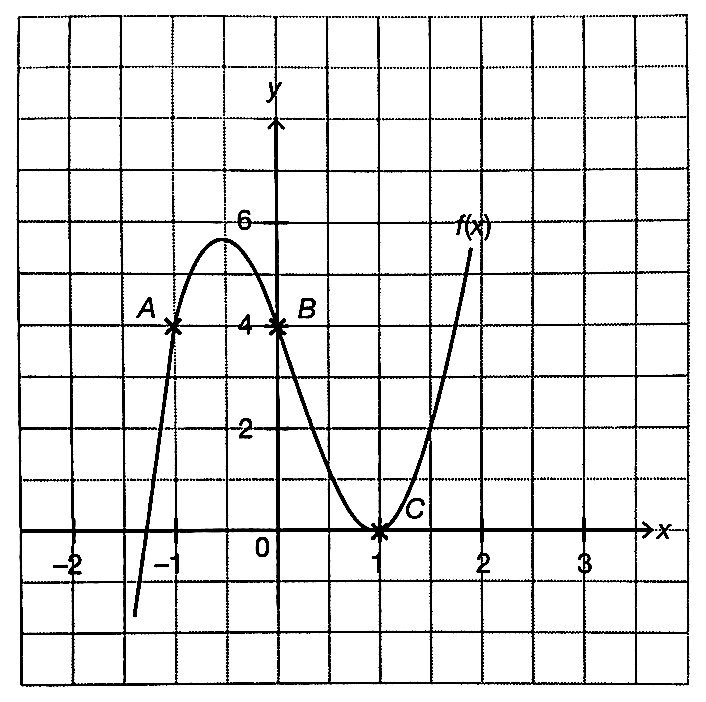
\includegraphics[width=0.3\textwidth]{./images/q24.jpeg}
                  \end{center}
                  \begin{enumerate}
                        \item Find the gradient function of the tangent to the curve $f(x)$. \sol{}
                              \begin{flalign*}
                                    f'(x) & = 9x^2 - 4x - 5 \eos
                              \end{flalign*}
                        \item \begin{enumerate}
                                    \item Find the values of gradient of the tangents to the curve at points $A$, $B$,
                                          and $C$. \sol{}
                                          \begin{flalign*}
                                                m_A & = f'(-1)                \\
                                                    & = 9{(-1)}^2 - 4(-1) - 5 \\
                                                    & = 9 + 4 - 5             \\
                                                    & = 8 \eos                \\
                                                m_B & = f'(0)                 \\
                                                    & = 9{(0)}^2 - 4(0) - 5   \\
                                                    & = -5 \eos               \\
                                                m_C & = f'(1)                 \\
                                                    & = 9{(1)}^2 - 4(1) - 5   \\
                                                    & = 9 - 4 - 5             \\
                                                    & = 0 \eos                \\
                                          \end{flalign*}

                                    \item Hence, elaborate the situations of the tangents at points $A$, $B$, and $C$
                                          based on the values of the gradient obtained in (i). \sol{}

                                          The gradient of the tangent at point $A$ is positive, hence the tangent is
                                          rising.

                                          The gradient of the tangent at point $B$ is negative, hence the tangent is
                                          falling.

                                          The gradient of the tangent at point $C$ is zero, hence the tangent is
                                          horizontal.
                              \end{enumerate}
                  \end{enumerate}
            \item Find the gradient of the tangent for each of the following curves at the given
                  point $P$.
                  \begin{enumerate}
                        \item $y = 4x - \dfrac{8}{x}; P(4, 14)$
                              \sol{}
                              \begin{flalign*}
                                    y' & = 4 - \dfrac{8}{x^2}     \\
                                       & = 4 + \dfrac{8}{x^2}     \\
                                       & = 4 + \dfrac{8}{{(4)}^2} \\
                                       & = 4 + \dfrac{1}{2}       \\
                                       & = 4.5 \eos
                              \end{flalign*}

                        \item $y = \dfrac{4 - 3x^2}{3-2x}; P(2, 8)$
                              \sol{}
                              \begin{flalign*}
                                    y' & = \dfrac{(3-2x)(-6x) - (4-3x^2)(-2)}{{(3-2x)}^2}         \\
                                       & = \frac{-18x + 12x^2 + 8 - 6x^2}{{(3-2x)}^2}             \\
                                       & = \frac{6x^2 -18x + 8}{{(3-2x)}^2}                       \\
                                       & = \frac{2(3x^2 - 9x + 4)}{{(3-2x)}^2}                    \\
                                       & = \frac{2\left[3{(2)}^2 - 9(2) + 4\right]}{{(3-2(2))}^2} \\
                                       & = -4 \eos
                              \end{flalign*}
                  \end{enumerate}

            \item \begin{enumerate}
                        \item Find the value of gradient of the tangent to the curve $y = 2x^3 - 3x^2$ when
                              $x = 1$. \sol{}
                              \begin{flalign*}
                                    \frac{dy}{dx} & = 6x^2 - 6x   \\
                                                  & = 6(1) - 6(1) \\
                                                  & = 0 \eos
                              \end{flalign*}

                        \item Find the coordinates of points to the curve $y = \dfrac{x^3}{3} + x^2 - 1$ such
                              that the gradient to the curve at the points is $8$. \sol{}
                              \begin{flalign*}
                                    \frac{dy}{dx}  & = x^2 + 2x        \\
                                    8              & = x^2 + 2x        \\
                                    x^2 + 2x - 8   & = 0               \\
                                    (x + 4)(x - 2) & = 0               \\
                                    x = -4         & \text{ or } x = 2
                              \end{flalign*}
                              When $x = -4$,
                              \begin{flalign*}
                                    y & = \dfrac{(-4)^3}{3} + (-4)^2 - 1 \\
                                      & = -\frac{64}{3} + 16 - 1         \\
                                      & = -\frac{19}{3}
                              \end{flalign*}
                              When $x = 2$,
                              \begin{flalign*}
                                    y & = \dfrac{2^3}{3} + 2^2 - 1 \\
                                      & = \frac{8}{3} + 4 - 1      \\
                                      & = \frac{17}{3}
                              \end{flalign*}
                              Therefore, the coordinates of the points are $(-4, -\dfrac{19}{3})$ and $(2, \dfrac{17}{3})$. $\eos$

                        \item Given the curve $y = ax^2 + bx + 3$ has the gradient $5$ when $x = 2$ and the
                              gradient $0$ when $x = -3$. Determine the values of $a$ and $b$. \sol{}
                              \begin{flalign*}
                                    \frac{dy}{dx}   & = 2ax + b                \\
                                    5               & = 2a(2) + b              \\
                                    4a + b          & = 5                & (1) \\
                                    0               & = 2a(-3) + b             \\
                                    -6a + b         & = 0                & (2) \\
                                    (1) - (2):\ 10a & = 5                      \\
                                    a               & = \frac{1}{2} \eos
                              \end{flalign*}
                              Substituting $a = \dfrac{1}{2}$ into (1),
                              \begin{flalign*}
                                    4\left(\dfrac{1}{2}\right) + b & = 5      \\
                                    b                              & = 3 \eos
                              \end{flalign*}
                  \end{enumerate}

            \item Find the equations of tangent and normal to the curve $y = 8 - 2x - x^2$ at
                  each of the following points. \sol{}
                  \begin{flalign*}
                        \frac{dy}{dx} & = -2 - 2x
                  \end{flalign*}
                  \begin{enumerate}
                        \item $A(1, 5)$
                              \sol{}

                              At point $A(1, 5)$, the gradient of the tangent is $-2 - 2(1) = -4$.

                              Hence, the equation of the tangent is
                              \begin{flalign*}
                                    y - 5 & = -4(x - 1)    \\
                                    y - 5 & = -4x + 4      \\
                                    y     & = -4x + 9 \eos
                              \end{flalign*}

                              At point $A(1, 5)$, the gradient of the normal is $\dfrac{1}{4}$.

                              Hence, the equation of the normal is
                              \begin{flalign*}
                                    y - 5       & = \dfrac{1}{4}(x - 1) \\
                                    4y - 20     & = x - 1               \\
                                    x - 4y + 19 & = 0 \eos
                              \end{flalign*}

                        \item $C(-1, 9)$
                              \sol{}

                              At point $C(-1, 9)$, the gradient of the tangent is $-2 - 2(-1) = 0$.

                              Hence, the equation of the tangent is
                              \begin{flalign*}
                                    y - 9 & = 0(x + 1) \\
                                    y - 9 & = 0        \\
                                    y     & = 9 \eos
                              \end{flalign*}

                              At point $C(-1, 9)$, the gradient of the normal is \textit{undefined}.

                              Hence, the equation of the normal is
                              \begin{flalign*}
                                    x + 1 & = 0       \\
                                    x     & = -1 \eos
                              \end{flalign*}
                  \end{enumerate}

            \item \begin{enumerate}
                        \item Find the equation of normal to the curve $y = 3x^2 + 8x - 7$ at point $(-2,
                                    6)$. \sol{}
                              \begin{flalign*}
                                    \frac{dy}{dx} & = 6x + 8
                              \end{flalign*}
                              The gradient of the tangent is $6(-2) + 8 = -4$.

                              The gradient of the normal is $\dfrac{1}{4}$.

                              Hence, the equation of the normal is
                              \begin{flalign*}
                                    y - 6       & = \dfrac{1}{4}(x + 2) \\
                                    4y - 24     & = x + 2               \\
                                    x - 4y + 26 & = 0 \eos
                              \end{flalign*}

                        \item Given the tangent to the curve $y = ax^2 + bx$ at the point $P(4, 8)$ is
                              perpendicular to the straight line that passes through the point $A(4, 1)$ and
                              the point $B(12, 0)$. Find the values of $a$ and $b$. \sol{}
                              \begin{flalign*}
                                    m_{AB} & = -\frac{1}{8}
                              \end{flalign*}
                              Since the tangent at point $P(4, 8)$ is perpendicular to the straight line $AB$,

                              The gradient of the tangent at point $P(4, 8)$ is $8$.
                              \begin{flalign*}
                                    \frac{dy}{dx} & = 2ax + b
                              \end{flalign*}
                              The gradient of the tangent at point $P(4, 8)$ is $2a(4) + b = 8a + b$.
                              \begin{flalign*}
                                    8a + b & = 8 \quad\cdots\quad (1)
                              \end{flalign*}
                              At point $P(4, 8)$
                              \begin{flalign*}
                                    a(4)^2 + b(4) & = 8                      \\
                                    16a + 4b      & = 8                      \\
                                    4a + b        & = 2 \quad\cdots\quad (2)
                              \end{flalign*}
                              \begin{flalign*}
                                    (1) - (2):\ 4a & = 6                \\
                                    a              & = \frac{3}{2} \eos
                              \end{flalign*}
                              Substituting $a = \dfrac{3}{2}$ into (2),
                              \begin{flalign*}
                                    b & = 2 - 4\left(\dfrac{3}{2}\right) \\
                                      & = 2 - 6                          \\
                                      & = -4 \eos
                              \end{flalign*}
                  \end{enumerate}

            \item Find the coordinates of the turning points for each of the following curves.
                  Hence, determine the nature of the turning points.
                  \begin{enumerate}
                        \item $y = 5x^2 - 2x + 1$
                              \sol{}
                              \begin{flalign*}
                                    \frac{dy}{dx} & = 10x - 2           \\
                                    10x - 2       & = 0                 \\
                                    10x           & = 2                 \\
                                    x             & = \dfrac{1}{5} \eos
                              \end{flalign*}
                              When $x = \dfrac{1}{5}$,
                              \begin{flalign*}
                                    y & = 5\left(\dfrac{1}{5}\right)^2 - 2\left(\dfrac{1}{5}\right) + 1 \\
                                      & = \dfrac{1}{5} - \dfrac{2}{5} + 1                               \\
                                      & = \dfrac{4}{5}
                              \end{flalign*}
                              Hence, the coordinates of the turning point are $\left(\dfrac{1}{5}, \dfrac{4}{5}\right)$. $\eos$
                              \begin{flalign*}
                                    \frac{d^2y}{dx^2} & = 10 > 0
                              \end{flalign*}
                              Hence, $\left(\dfrac{1}{5}, \dfrac{4}{5}\right)$ is a \textit{maximum point}. $\eos$

                        \item $y = \dfrac{x^2}{x+1}$
                              \sol{}
                              \begin{flalign*}
                                    \frac{dy}{dx}                 & = \dfrac{(x+1)(2x) - x^2}{{(x+1)}^2} \\
                                                                  & = \dfrac{2x^2 + 2x - x^2}{{(x+1)}^2} \\
                                                                  & = \dfrac{x(x+2)}{{(x+1)}^2}          \\
                                    \dfrac{x(x+2)}{{(x+1)}^2}     & = 0                                  \\
                                    x(x+2)                        & = 0                                  \\
                                    x                         = 0 & \text{ or } x = -2
                              \end{flalign*}
                              When $x = 0$,
                              \begin{flalign*}
                                    y & = \dfrac{0^2}{0+1} \\
                                      & = 0
                              \end{flalign*}
                              When $x = -2$,
                              \begin{flalign*}
                                    y & = \dfrac{{(-2)}^2}{(-2)+1} \\
                                      & = \dfrac{4}{-1}            \\
                                      & = -4
                              \end{flalign*}
                              Hence, the coordinates of the turning points are $\left(0, 0\right)$ and $\left(-2, -4\right)$. $\eos$
                              \begin{flalign*}
                                    \frac{dy}{dx}     & = \dfrac{x^2+2x}{{(x+1)}^2}                               \\
                                    \frac{d^2y}{dx^2} & = \dfrac{(2x + 2){(x+1)}^2 - 2(x+1)(x^2 + 2x)}{{(x+1)}^4} \\
                                                      & = \frac{(x+1)[(2x+2)(x+1) - 2(x^2 + 2x)]}{{(x+1)}^4}      \\
                                                      & = \frac{2x^2 + 4x + 2 - 2x^2 - 4x}{{(x+1)}^3}             \\
                                                      & = \frac{2}{{(x+1)}^3}
                              \end{flalign*}
                              When $x = 0$,
                              \begin{flalign*}
                                    \frac{d^2y}{dx^2} & = \frac{2}{{(0+1)}^3} \\
                                                      & = \frac{2}{1^3}       \\
                                                      & = 2 > 0
                              \end{flalign*}
                              Hence, $\left(0, 0\right)$ is a \textit{maximum point}. $\eos$

                              When $x = -2$,
                              \begin{flalign*}
                                    \frac{d^2y}{dx^2} & = \frac{2}{{(-2+1)}^3} \\
                                                      & = \frac{2}{(-1)^3}     \\
                                                      & = -2 < 0
                              \end{flalign*}
                              Hence, $\left(-2, -4\right)$ is a \textit{minimum point}. $\eos$

                        \item $y = 7 - x^3$
                              \sol{}
                              \begin{flalign*}
                                    \frac{dy}{dx} & = -3x^2 \\
                                    -3x^2         & = 0     \\
                                    x             & = 0
                              \end{flalign*}
                              When $x = 0$,
                              \begin{flalign*}
                                    y & = 7 - 0^3 \\
                                      & = 7
                              \end{flalign*}
                              Hence, the coord. of the turning point is $\left(0, 7\right)$. $\eos$
                              \begin{flalign*}
                                    \frac{d^2y}{dx^2} & = -6x
                              \end{flalign*}
                              When $x = 0$,
                              \begin{flalign*}
                                    \frac{d^2y}{dx^2} & = -6(0) \\
                                                      & = 0
                              \end{flalign*}
                              Hence, $\left(0, 7\right)$ is a \textit{inflection point}. $\eos$
                  \end{enumerate}

            \item Solve the following problems related to stationary points.
                  \begin{enumerate}
                        \item The following diagram shows the plan of a cuboid in which its centre in the
                              shape of a cylinder is taken out. The cuboid measures $3x\textit{cm} \times
                                    2x\textit{cm} \times (45 - 5x)\textit{cm}$.
                              \begin{center}
                                    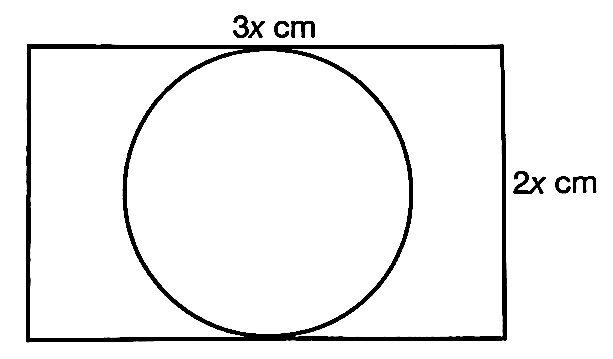
\includegraphics[width=0.3\textwidth]{./images/q30.jpeg}
                              \end{center}
                              Find the value of $x$ that makes the volume of the cylinder taken out a maximum.
                              \sol{}
                              \begin{flalign*}
                                    r & = x                    \\
                                    V & = \pi r^2h             \\
                                      & = \pi x^2(45 - 5x)     \\
                                      & = 45\pi x^2 - 5\pi x^3
                              \end{flalign*}
                              $V$ is maximum when
                              \begin{flalign*}
                                    \frac{dV}{dx}            & = 0                \\
                                    90\pi x - 15\pi x^2      & = 0                \\
                                    6x - x^2                 & = 0                \\
                                    x(x-6)                   & = 0                \\
                                    x                   = 0  & \text{ or } x = 6  \\
                                    x \neq 0                 & ,\ x = 6           \\
                                    x = 6, \frac{d^2V}{dx^2} & = 90\pi - 30\pi(6) \\
                                                             & = 90\pi - 180\pi   \\
                                                             & = -90\pi < 0
                              \end{flalign*}
                              Hence, $x = 6$ is the value of $x$ that makes the volume of the cylinder taken out a maximum. $\eos$

                        \item Given $A = bh$ where $b^2 + h^2 = 40$ and $b, h > 0$. Find the values of $b$
                              and $h$ so that $A$ becomes a stationary point and show that the value of $A$
                              is maximum. \sol{}
                              \begin{flalign*}
                                    b^2 + h^2 & = 40                          \\
                                    b^2       & = 40 - h^2                    \\
                                    b         & = \sqrt{40 - h^2}             \\
                                              & = {(40 - h^2)}^{\frac{1}{2}}  \\
                                    A         & = bh                          \\
                                              & = {(40 - h^2)}^{\frac{1}{2}}h
                              \end{flalign*}
                              $A$ is stationary when
                              \begin{flalign*}
                                    \frac{dA}{dh}                                    & = 0                                      & \\
                                    -\frac{2h^2}{2\sqrt{40 - h^2}} + \sqrt{40 - h^2} & = 0                                        \\
                                    -\frac{2h^2}{2\sqrt{40 - h^2}} + \sqrt{40 - h^2} & = 0                                        \\
                                    \frac{-h^2 + 40 - h^2}{\sqrt{40 - h^2}}          & = 0                                        \\
                                    -2h^2 + 40                                       & = 0                                        \\
                                    h^2                                              & = 20                                       \\
                                    h                                                & = \sqrt{20}\ (h > 0) \eos                  \\
                                    b                                                & = \sqrt{40 - {\left(\sqrt{20}\right)}^2}   \\
                                                                                     & = \sqrt{20} \eos
                              \end{flalign*}
                              \begin{flalign*}
                                    A = \sqrt{20} \cdot \sqrt{20} & = 20
                              \end{flalign*}
                              \begin{center}
                                    \setcellgapes{2ex}\makegapedcells
                                    \begin{tabular}{|p{10em}|c|c|c|}
                                          \hline
                                          $h$              & $4$                                 & $\sqrt{20}$ & $5$          \\
                                          \hline
                                          $\dfrac{dA}{dh}$ & $1.63$                              & $0$         & $-2.58$      \\
                                          \hline
                                          Tangent Sketch   & $/$                                 & $-$         & $\backslash$ \\
                                          \hline
                                          Graph Sketch     & \multicolumn{3}{c|}{$/-\backslash$}                              \\
                                          \hline
                                    \end{tabular}
                              \end{center}
                              Hence, $A = 20$ is maximum when $h = \sqrt{20}$. $\eos$

                        \item A piece of wire with a length of $120\textit{cm}$ is divided into two parts
                              where is each is bent to form an equilateral triangle with an edge of
                              $x\textit{cm}$ and a square with an edge of $y\textit{cm}$ respectively.
                              Express $y$ in terms of $x$. Hence, show that the total area of both shapes,
                              $A\textit{cm}^2$ is given by
                              \[A = \dfrac{9{(40 - x)}^2 + 4\sqrt{3}x^2}{16}\]
                              Calculate the value of $x$ so that $A$ has a stationary value. Determine
                              whether this value of $x$ makes $A$ a maximum of a minimum. \sol{}
                              \begin{flalign*}
                                    C_\textit{triangle} & = 3x                 \\
                                    C_\textit{square}   & = 4y                 \\
                                    3x + 4y             & = 120                \\
                                    y                   & = \frac{120 - 3x}{4}
                              \end{flalign*}
                              \begin{flalign*}
                                    A_\textit{triangle} & = \dfrac{1}{2}bh                                                  & \\
                                                        & = \dfrac{1}{2}x\sqrt{x^2 - {\left(\frac{x}{2}\right)}^2}            \\
                                                        & = \dfrac{1}{2}x\sqrt{x^2 - \frac{x^2}{4}}                           \\
                                                        & = \dfrac{1}{2}x\sqrt{\frac{3x^2}{4}}                                \\
                                                        & = \dfrac{1}{2}x\left(\frac{1}{2}x\sqrt{3}\right)                    \\
                                                        & = \dfrac{\sqrt{3}x^2}{4}                                            \\
                                    A_\textit{square}   & = y^2                                                               \\
                                                        & = {\left(\frac{120 - 3x}{4}\right)}^2                               \\
                                                        & = \frac{{(120 - 3x)}^2}{16}                                         \\
                                                        & = \frac{{[3(40 - x)]}^2}{16}                                        \\
                                                        & = \frac{9{(40 - x)}^2}{16}                                          \\
                                    A                   & = A_\textit{square} + A_\textit{triangle}                           \\
                                                        & = \frac{9{(40 - x)}^2}{16} + \frac{\sqrt{3}x^2}{4}                  \\
                                                        & = \frac{9{(40 - x)}^2 + 4\sqrt{3}x^2}{16}\quad (\text{shown})\eos
                              \end{flalign*}
                              $A$ is stationary when $\dfrac{dA}{dx} = 0$.
                              \begin{flalign*}
                                    \frac{dA}{dx} & = \frac{d}{dx}\left[\frac{9{(40 - x)}^2 + 4\sqrt{3}x^2}{16}\right]          & \\
                                                  & = \frac{d}{dx}\left[\frac{9{(40 - x)}^2}{16} + \frac{\sqrt{3}x^2}{4}\right]   \\
                                                  & = \frac{-18(40 - x)}{16} + \frac{2\sqrt{3}x}{4}                               \\
                                                  & = -\frac{9(40 - x)}{8} + \frac{4\sqrt{3}x}{8}                                 \\
                                                  & = -\frac{9(40 - x) - 4\sqrt{3}x}{8}
                              \end{flalign*}
                              \begin{flalign*}
                                    -\frac{9(40 - x) - 4\sqrt{3}x}{8} & = 0                          \\
                                    360 - 9x - 4\sqrt{3}x             & = 0                          \\
                                    9x + 4\sqrt{3}x                   & = 360                        \\
                                    \left(9 + 4\sqrt{3}\right)x       & = 360                        \\
                                    x                                 & = \frac{360}{9 + 4\sqrt{3}}  \\
                                                                      & \approx 22.6\textit{cm} \eos
                              \end{flalign*}
                              \begin{flalign*}
                                    \frac{d^2A}{dx^2} & = \frac{9 + 4\sqrt{3}}{8} > 0
                              \end{flalign*}
                              Hence, $A$ is a minimum when $x = 22.6\textit{cm}$. $\eos$

                        \item Chan wants to build two separate pens by using a fence of $100\textit{m}$. Both
                              pens are square in shape.
                              \begin{center}
                                    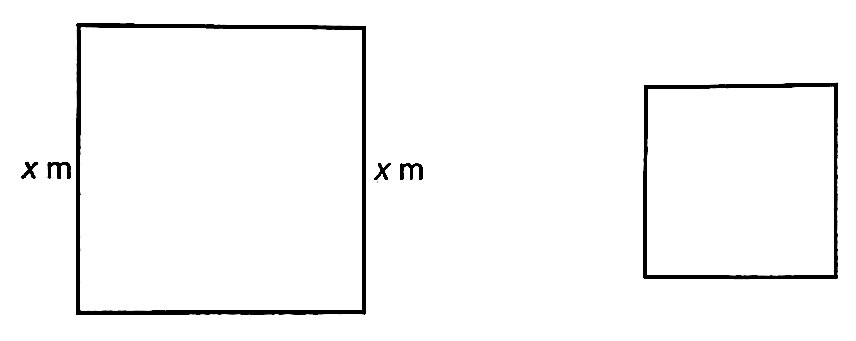
\includegraphics[width=0.4\textwidth]{./images/q30_2.jpeg}
                              \end{center}
                              If the edge of the larger pen is $x\textit{m}$,
                              \begin{enumerate}
                                    \item find the length of the side of the smaller pen in terms of $x$. \sol{} Let the
                                          length of the side of the smaller pen be $y\textit{m}$.
                                          \begin{flalign*}
                                                C_\textit{larger}  & = 4x                                     \\
                                                C_\textit{smaller} & = 4y                                     \\
                                                C_\textit{fence}   & = C_\textit{larger} + C_\textit{smaller} \\
                                                100                & = 4x + 4y                                \\
                                                25                 & = x + y                                  \\
                                                y                  & = (25 - x)\textit{m} \eos
                                          \end{flalign*}
                                    \item find the value of $x$ such that the total area of both pens is minimum. \sol{}
                                          \begin{flalign*}
                                                A_\textit{larger}  & = x^2                                    \\
                                                A_\textit{smaller} & = y^2                                    \\
                                                                   & = {(25 - x)}^2                           \\
                                                A                  & = A_\textit{larger} + A_\textit{smaller} \\
                                                                   & = x^2 + {(25 - x)}^2
                                          \end{flalign*}
                                          $A_\textit{total}$ is stationary when
                                          \begin{flalign*}
                                                \frac{dA}{dx}  & = 0                   \\
                                                2x - 2(25 - x) & = 0                   \\
                                                2x - 50 + 2x   & = 0                   \\
                                                4x             & = 50                  \\
                                                x              & = 12.5\textit{m} \eos
                                          \end{flalign*}
                                          \begin{flalign*}
                                                \frac{d^2A}{dx^2} & = 4 > 0
                                          \end{flalign*}
                                          Hence, $A$ is a minimum when $x = 12.5\textit{m}$. $\eos$
                              \end{enumerate}
                  \end{enumerate}

            \item Solve the following problems related to the rates of change.
                  \begin{enumerate}
                        \item The total surface area, $A\textit{cm}^2$, of a metal solid which consists of a
                              cone and a cylinder with a common radius, $r\textit{cm}$ is given by $A =
                                    2\pi\left(\dfrac{18}{r} + \dfrac{r^2}{3}\right)$. When it is heated, its total
                              surface area changes at the rate of $2.1\pi \textit{cm}^2\textit{s}^{-1}$. Find
                              the rate of change of the radius, in $\textit{cm} \textit{s}^{-1}$, at the
                              instant $r = 6\textit{cm}$. \sol{}
                              \begin{flalign*}
                                    A             & = 2\pi\left(\dfrac{18}{r} + \dfrac{r^2}{3}\right)                       \\
                                    \frac{dA}{dr} & = 2\pi\left(-\dfrac{18}{r^2} + \dfrac{2r}{3}\right)                     \\
                                    \frac{dA}{dt} & = 2.1\pi                                                                \\
                                    \frac{dr}{dt} & = \frac{dr}{dA} \cdot \frac{dA}{dt}                                     \\
                                    \frac{dA}{dt} & = \frac{dA}{dr} \cdot \frac{dr}{dt}                                     \\
                                    2.1\pi        & = 2\pi\left(-\dfrac{18}{r^2} + \dfrac{2r}{3}\right) \cdot \frac{dr}{dt} \\
                                    \frac{dr}{dt} & = \frac{2.1}{2\left(-\dfrac{18}{r^2} + \dfrac{2r}{3}\right)}            \\
                                                  & = \frac{2.1}{2\left(-\dfrac{18}{6^2} + \dfrac{2(6)}{3}\right)}          \\
                                                  & = 0.3\textit{cm}\textit{s}^{-1}
                              \end{flalign*}

                        \item A spherical balloon experiences a constant rate of increase of
                              $6\textit{cm}^2\textit{s}^{-1}$.
                              \begin{center}
                                    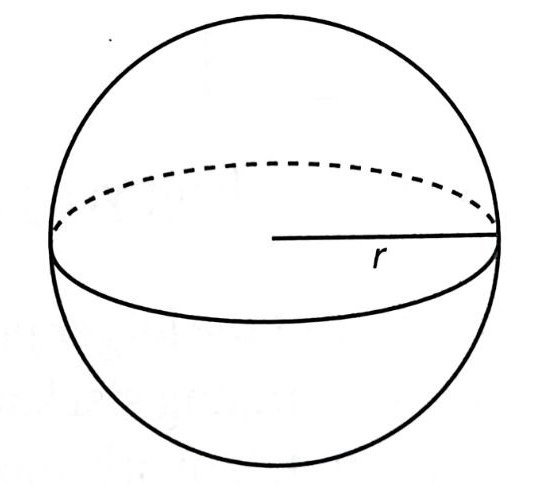
\includegraphics[width=0.3\textwidth]{./images/q31.jpeg}
                              \end{center}
                              At the instant when the radius is 5\textit{cm}, find
                              \begin{enumerate}
                                    \item the rate of increase, in $\textit{cm} \textit{s}^{-1}$, of the radius. \sol{}
                                          \begin{flalign*}
                                                S             & = 4\pi r^2                                   \\
                                                \frac{dS}{dr} & = 8\pi r                                     \\
                                                \frac{dS}{dt} & = 6                                          \\
                                                \frac{dr}{dt} & = \frac{dr}{dS} \cdot \frac{dS}{dt}          \\
                                                \frac{dS}{dt} & = \frac{dr}{dt} \cdot \frac{dS}{dr}          \\
                                                6             & = \frac{dr}{dt} \cdot 8\pi r                 \\
                                                \frac{dr}{dt} & = \frac{3}{4\pi r}                           \\
                                                              & = \frac{3}{20\pi} \textit{cm}\textit{s}^{-1}
                                          \end{flalign*}

                                    \item the rate of increase if volume, in $\textit{cm}^3 \textit{s}^{-1}$, of the
                                          sphere. \sol{}
                                          \begin{flalign*}
                                                V             & = \frac{4}{3}\pi r^3                \\
                                                \frac{dV}{dr} & = 4\pi r^2                          \\
                                                \frac{dV}{dt} & = \frac{dV}{dr} \cdot \frac{dr}{dt} \\
                                                              & = 4\pi r^2 \cdot \frac{3}{4\pi r}   \\
                                                              & = 3r                                \\
                                                              & = 3(5)                              \\
                                                              & = 15\textit{cm}^3\textit{s}^{-1}
                                          \end{flalign*}
                              \end{enumerate}

                        \item The following diagram shows a container in the shape of a cone. Given its
                              height is equal to its base radius. Water is poured into the container at the
                              rate of $80\textit{cm}^3\textit{s}^{-1}$. The volume of the water in the
                              container is $\dfrac{1}{3}\pi x^3\textit{cm}^3$, when the depth of the water is
                              $x\textit{cm}$.
                              \begin{center}
                                    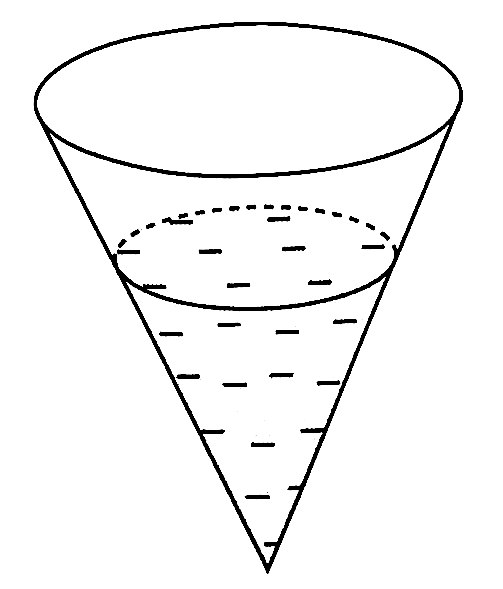
\includegraphics[width=0.2\textwidth]{./images/q31_2.jpeg}
                              \end{center}
                              Calculate, at the instant when the depth of the water is $10\textit{cm}$,
                              \begin{enumerate}
                                    \item the rate of increase of the depth, in $\textit{cm} \textit{s}^{-1}$, of the
                                          water. \sol{}

                                          At time $t$, let $V = $ volume of water
                                          \begin{flalign*}
                                                \frac{dV}{dt} & = 80                                        \\
                                                \frac{dV}{dx} & = \pi x^2                                   \\
                                                \frac{dx}{dt} & = \frac{dx}{dV} \cdot \frac{dV}{dt}         \\
                                                \frac{dV}{dt} & = \frac{dx}{dt} \cdot \frac{dV}{dx}         \\
                                                80            & = \frac{dx}{dt} \cdot \pi x^2               \\
                                                \frac{dx}{dt} & = \frac{80}{\pi x^2}                        \\
                                                              & = \frac{80}{\pi{(10)}^2}                    \\
                                                              & = \frac{4}{5\pi} \textit{cm}\textit{s}^{-1}
                                          \end{flalign*}

                                    \item the rate of increase of the horizontal surface area, in $\textit{cm}^2
                                                \textit{s}^{-1}$, of the water.

                                          At time $t$, let

                                          $A = $ horizontal surface area of water

                                          $r = $ radius of the water surface

                                          $R = $ radius of the base of the container

                                          $h = $ height of the container
                                          \begin{flalign*}
                                                R             & = h \quad (\text{given})            \\
                                                \frac{r}{R}   & = \frac{x}{h}                       \\
                                                \frac{r}{h}   & = \frac{x}{h}                       \\
                                                r             & = x                                 \\
                                                A             & = \pi rx                            \\
                                                              & = \pi x^2                           \\
                                                \frac{dA}{dx} & = 2\pi x                            \\
                                                \frac{dA}{dt} & = \frac{dA}{dx} \cdot \frac{dx}{dt} \\
                                                              & = 2\pi x \cdot \frac{80}{\pi x^2}   \\
                                                              & = \frac{160}{x}                     \\
                                                              & = \frac{160}{10}                    \\
                                                              & = 16\textit{cm}^2\textit{s}^{-1}
                                          \end{flalign*}
                              \end{enumerate}
                  \end{enumerate}

            \item Solve the following problems related to the small changes and approximations.
                  \begin{enumerate}
                        \item Given that $y = 2x^3 - 5x^2 + x - 1$, find the value of $\dfrac{dy}{dx}$ when
                              $x = 1$. Hence, find the small changes in $y$ when $x$ increases from $1$ to
                              $1.02$. \sol{}
                              \begin{flalign*}
                                    \frac{dy}{dx} & = 6x^2 - 10x + 1
                              \end{flalign*}
                              When $x = 1$, $\frac{dy}{dx} = 6{(1)}^2 - 10(1) + 1 = -3$. $\eos$
                              \begin{flalign*}
                                    y_{\textit{new}}          & = y_{\textit{original}} + \delta y                     \\
                                                              & = y_{\textit{original}} + \frac{dy}{dx} \cdot \delta x \\
                                    \frac{\delta y}{\delta x} & \approx \frac{dy}{dx}                                  \\
                                    \delta y                  & \approx \frac{dy}{dx} \cdot \delta x                   \\
                                                              & = -3 \cdot (1.02 - 1)                                  \\
                                                              & = -0.06
                              \end{flalign*}

                        \item Given the equation of a curve is $y = \dfrac{9}{{(2x - 5)}^2}$, find, in terms
                              of $p$, where $p$ is a small value, the approximate change in \sol{}
                              \begin{flalign*}
                                    \frac{dy}{dx} & = \frac{0 - 9(2)(2x-5)(2)}{{(2x-5)}^4} \\
                                                  & = \frac{-36(2x-5)}{{(2x-5)}^4}         \\
                                                  & = -\frac{36}{{(2x-5)}^3}
                              \end{flalign*}
                              \begin{enumerate}
                                    \item $y$ when $x$ increases from $3$ to $3 + p$.
                                          \sol{}
                                          When $x = 3$,
                                          \begin{flalign*}
                                                \frac{\delta y}{\delta x} & \approx \frac{dy}{dx}                  \\
                                                \delta y                  & \approx \frac{dy}{dx} \cdot \delta x   \\
                                                                          & = -\frac{36}{{(2x-5)}^3} \cdot (3+p-3) \\
                                                                          & = -\frac{36}{{(2(3)-5)}^3} \cdot p     \\
                                                                          & = -36p \eos
                                          \end{flalign*}

                                    \item $x$ when $y$ decreases from $1$ to $1 - p$.
                                          \sol{}
                                          When $y = 1$,
                                          \begin{flalign*}
                                                \frac{9}{{(2x-5)}^2} & = 1                 \\
                                                {(2x-5)}^2           & = 9                 \\
                                                2x-5                 & = \pm 3             \\
                                                x                    & = \frac{5 \pm 3}{2} \\
                                                x = 4                & \text{ or } x = 1
                                          \end{flalign*}
                                          \begin{flalign*}
                                                \frac{\delta y}{\delta x} & \approx \frac{dy}{dx}
                                          \end{flalign*}
                                          When $x = 1$,
                                          \begin{flalign*}
                                                \frac{-p}{\delta x} & = -\frac{36}{{(2(1)-5)}^3} \\
                                                                    & = \frac{4}{3}
                                          \end{flalign*}
                                          When $x = 4$,
                                          \begin{flalign*}
                                                \frac{-p}{\delta x} & = -\frac{36}{{(2(4)-5)}^3} \\
                                                                    & = -\frac{4}{3}
                                          \end{flalign*}
                                          Hence,
                                          \begin{flalign*}
                                                \frac{-p}{\delta x} & = \pm\frac{4}{3}                \\
                                                -p                  & = \pm\frac{4}{3} \cdot \delta y \\
                                                \delta y            & = \pm{\frac{3}{4}}p \eos
                                          \end{flalign*}
                              \end{enumerate}

                        \item Given $y = x^4$, by using the calculus method, find the approximate value of
                              \sol{}
                              \begin{flalign*}
                                    \frac{dy}{dx} & = 4x^3 \\
                              \end{flalign*}
                              When $x = 2$, $\frac{dy}{dx} = 4{(2)}^3 = 32$.
                              \begin{enumerate}
                                    \item $2.03^4$.
                                          \begin{flalign*}
                                                y_{\textit{new}} & = y_{\textit{original}} + \delta y                     \\
                                                                 & = y_{\textit{original}} + \frac{dy}{dx} \cdot \delta x
                                          \end{flalign*}
                                          \begin{flalign*}
                                                {(2.03)}^4 & = {(2)}^4 + 4{(2)}^3 \cdot (2.03 - 2) \\
                                                           & = 16 + 32(0.03)                       \\
                                                           & = 16 + 0.96                           \\
                                                           & = 16.96 \eos
                                          \end{flalign*}

                                    \item $1.99^4$.
                                          \begin{flalign*}
                                                y_{\textit{new}} & = y_{\textit{original}} + \delta y                     \\
                                                                 & = y_{\textit{original}} + \frac{dy}{dx} \cdot \delta x
                                          \end{flalign*}
                                          \begin{flalign*}
                                                {(1.99)}^4 & = {(2)}^4 - 4{(2)}^3 \cdot (2 - 1.99) \\
                                                           & = 16 - 32(0.01)                       \\
                                                           & = 16 - 0.32                           \\
                                                           & = 15.68 \eos
                                          \end{flalign*}
                              \end{enumerate}
                  \end{enumerate}

            \item A hemispherical bowl of radius $R\textit{cm}$ is filled with water to a depth
                  of $h\textit{cm}$.
                  \begin{center}
                        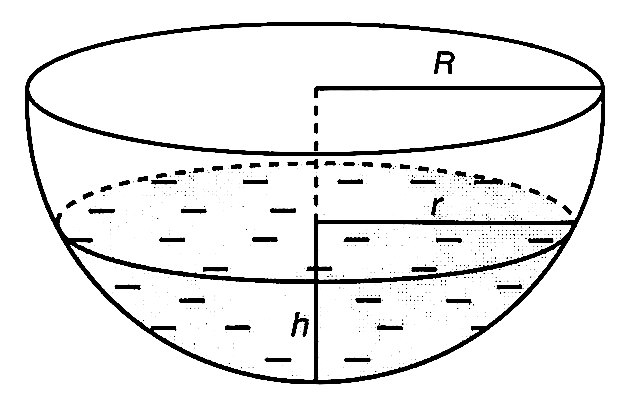
\includegraphics[width=0.3\textwidth]{./images/q33.jpeg}
                  \end{center}
                  The volume of the water in the bowl is given by $V = \dfrac{\pi}{3}(3Rh^2 - h^3)$.
                  \begin{enumerate}
                        \item Show that the radius of the water surface, $r$, is given by $r = \sqrt{2Rh -
                                          h^2}$. \sol{}
                              \begin{flalign*}
                                    R^2 & = r^2 + {(R - h)}^2]                 \\
                                        & = r^2 + R^2 - 2Rh + h^2              \\
                                    r^2 & = R^2 - R^2 + 2Rh - h^2              \\
                                        & = 2Rh - h^2                          \\
                                    r   & = \sqrt{2Rh - h^2}\quad (r > 0) \eos
                              \end{flalign*}

                        \item Water is poured into the bown at a constand rate of
                              $300\textit{cm}^3\textit{min}^{-1}$. Find, in terms of $R$, the rate of
                              increase of the surface area, in $\textit{cm}^2 \textit{min}^{-1}$, of the
                              water when $2h = R$. \sol{}
                              \begin{flalign*}
                                    V             & = \frac{\pi}{3}(3Rh^2 - h^3)                            \\
                                                  & = \frac{\pi}{3}(6h^3 - h^3) \quad (2h = R)              \\
                                                  & = \frac{5}{3}h^3\pi                                     \\
                                    \frac{dV}{dh} & = 5h^2\pi                                               \\
                                    \frac{dV}{dt} & = 300                                                   \\
                                    A             & = \pi r^2                                               \\
                                                  & = \pi (2Rh - h^2)                                       \\
                                                  & = \pi (4h^2 - h^2) \quad (2h = R)                       \\
                                                  & = 3h^2\pi                                               \\
                                    \frac{dA}{dh} & = 6h\pi                                                 \\
                                    \frac{dA}{dt} & = \frac{dA}{dh} \cdot \frac{dh}{dV} \cdot \frac{dV}{dt} \\
                                                  & = 6h\pi \cdot \frac{1}{5h^2\pi} \cdot 300               \\
                                                  & = \frac{360}{h}                                         \\
                                                  & = \frac{360}{\frac{R}{2}} \quad (2h = R)                \\
                                                  & = \frac{720}{R} \textit{cm}^2 \textit{min}^{-1} \eos
                              \end{flalign*}
                  \end{enumerate}
      \end{enumerate}
\end{multicols*}
\begin{multicols*}{2}
      \noindent\Large{\underline{\textbf{Praktis Summatif}}}
      \normalsize
      \setcounter{section}{0}
      \section{Kertas 1}
      \begin{enumerate}
            \item Given $\delta y = 4x \delta x + 2{(\delta x)}^2 + 3 \delta x$. Find
                  $\dfrac{dy}{dx}$ when $x = 2$. \sol{}
                  \begin{flalign*}
                        \delta y                  & = 4x \delta x + 2{(\delta x)}^2 + 3 \delta x    \\
                        \frac{\delta y}{\delta x} & = 4x  + 2\delta x + 3                           \\
                        \frac{dy}{dx}             & = \lim_{\delta x\to 0}\frac{\delta y}{\delta x} \\
                                                  & =  \lim_{\delta x\to 0}(4x  + 2\delta x + 3)    \\
                                                  & = 4x + 3
                  \end{flalign*}
                  When $x = 2$, $\dfrac{dy}{dx} = 4(2) + 3 = 11$. $\eos$

            \item Given $\dfrac{d}{dx}\left(\dfrac{x^3}{3-x^3}\right) =
                        \dfrac{kx^m}{{(3-x^3)}^n}$, determine the values of $k$, $m$, and $n$. \sol{}
                  \begin{flalign*}
                        \dfrac{d}{dx}\left(\dfrac{x^3}{3-x^3}\right) & = \frac{(3-x^3)(3x^2) - (x^3)(-3x^2)}{{(3-x^3)}^2} \\
                                                                     & = \frac{9x^2}{{(3-x^3)}^2}                         \\
                        \frac{kx^m}{{(3-x^3)}^n}                     & = \frac{9x^2}{{(3-x^3)}^2}                         \\
                  \end{flalign*}
                  Comparing both sides, $k = 9$, $m = 2$, and $n = 2$. $\eos$

            \item In the diagram in the answer space, sketch a graph $y = f(x)$ that satisfies
                  the following conditions:
                  \begin{enumerate}
                        \item The points $A(x_a, y_a)$, $B(x_b, y_b)$, and $C(x_c, y_c)$ lies on the curve
                              $y$.
                        \item $f'(x_a) = f'(x_b) = f'(x_c) = 0$.
                        \item $f''(x_c) < f''(x_b) < f''(x_a)$.
                        \item $f''(x_b) = 0$.
                              \sol{}
                              \begin{center}
                                    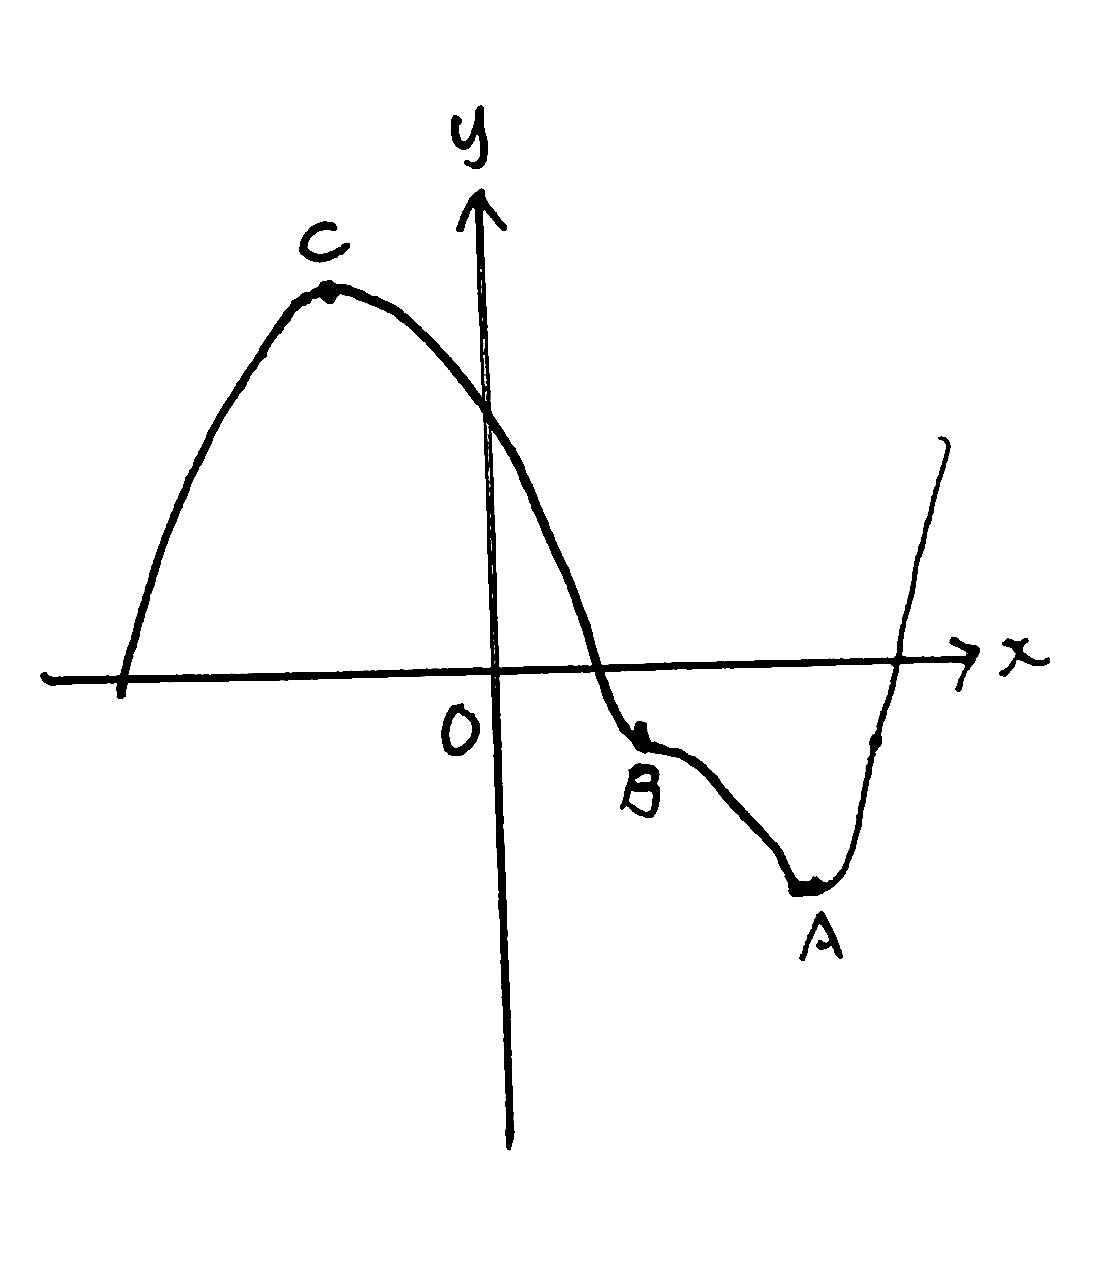
\includegraphics[width=0.3\textwidth]{./images/k1q2.jpeg}
                              \end{center}
                  \end{enumerate}

            \item \begin{enumerate}
                        \item Find $\lim\limits_{x\to3}\dfrac{x-3}{4-\sqrt{19-x}}$. \sol{}
                              \begin{flalign*}
                                    \lim\limits_{x\to3}\dfrac{x-3}{4-\sqrt{19-x}} & = \lim\limits_{x\to3}\dfrac{(x-3)'}{(4-\sqrt{19-x})'}   \\
                                                                                  & = \lim\limits_{x\to3}\dfrac{1}{\dfrac{1}{2\sqrt{19-x}}} \\
                                                                                  & = \lim\limits_{x\to3}\left(2\sqrt{19-x}\right)          \\
                                                                                  & = 2\sqrt{19-3}                                          \\
                                                                                  & = 8 \eos
                              \end{flalign*}

                        \item Given $y = 5$ and $\frac{dy}{dx} = kx^m$. Based on the formula for the first
                              derivative, state the value of $k$ and $m$. \sol{}
                              \begin{flalign*}
                                    y             & = 5           \\
                                                  & = 5x^{0}      \\
                                    \frac{dy}{dx} & = (0)5x^{0-1} \\
                                                  & = 0x^{-1}     \\
                                    kx^m          & = 0x^{-1}
                              \end{flalign*}
                              Comparing both sides, $k = 0$ and $m = -1$. $\eos$
                  \end{enumerate}

            \item Given the equation of a curve $y = 2x^2 + 7x -1$. Find the coordinates of a
                  point on the curve that has a gradient of $5$. Hence, find the value of
                  constant $p$ such that $y = 5x + p$ is the tangent to the curve. \sol{}
                  \begin{flalign*}
                        \frac{dy}{dx} & = 4x + 7                                                          \\
                        4x + 7        & = 5                                                               \\
                        4x            & = -2                                                              \\
                        x             & = -\frac{1}{2}                                                    \\
                        y             & = 2{\left(-\frac{1}{2}\right)}^2 + 7\left(-\frac{1}{2}\right) - 1 \\
                                      & = 0.5 - 3.5 - 1                                                   \\
                                      & = -4
                  \end{flalign*}
                  Hence, the coordinates of the point is $\left(-\frac{1}{2}, -4\right)$. $\eos$

            \item Show that the gradient of the curve $y = 3x^3 - 18x^2 + 42x - 29$ is never
                  negative for all the values of $x$. \prooff{}
                  \begin{flalign*}
                        \frac{dy}{dx} & = 9x^2 - 36x + 42       \\
                                      & = 9(x^2 - 4x) + 42      \\
                                      & = 9[{(x-2)}^2 - 4] + 42 \\
                                      & = 9{(x-2)}^2 - 36 + 42  \\
                                      & = 9{(x-2)}^2 + 6
                  \end{flalign*}
                  \begin{flalign*}
                        \because\    & \forall x \in \mathbb{R},\ {(x-2)}^2 + 6 \geq 0 \\
                        \therefore\  & \forall x \in \mathbb{R},\ \frac{dy}{dx} \geq 0
                  \end{flalign*}
      \end{enumerate}

      \section{Kertas 2}
      \begin{enumerate}
            \item Given the equation of a curve $y = 2x^3 + x$. By using the differentiation
                  method, find in terms of $p$, the approximate percentage increase in $y$ when
                  $x$ increases from $2$ by $p\%$, where $p$ is a small value. \sol{}
                  \begin{flalign*}
                        \frac{dy}{dx} & = 6x^2 + 1
                  \end{flalign*}
                  When $x = 2$, $\dfrac{dy}{dx} = 25$.
                  \begin{flalign*}
                        \frac{\delta y}{\delta x} & \approx \dfrac{dy}{dx}                 \\
                        \delta y                  & \approx \dfrac{dy}{dx}\cdot \delta x   \\
                                                  & = 25 \cdot \dfrac{p}{100} \cdot 2      \\
                                                  & = 0.5p                                 \\
                        \% \delta y               & = \dfrac{\delta y}{y} \cdot 100        \\
                                                  & = \dfrac{0.5p}{2{(2)}^3 + 2} \cdot 100 \\
                                                  & = \dfrac{0.5p}{18} \cdot 100           \\
                                                  & = \frac{25}{9}p \eos
                  \end{flalign*}

            \item A curve $y_1 = x^2 - x - 5$ intersects another curve $y_2 = x^2 - \frac{31}{5}x
                        + \frac{53}{5}$ at point $A$.
                  \begin{enumerate}
                        \item Determine the gradient functions for both curves at the point of intersection
                              $A$. \sol{}
                              \begin{flalign*}
                                    y_1           & = y^2                                \\
                                    x^2 - x - 5   & = x^2 - \frac{31}{5}x + \frac{53}{5} \\
                                    5x + 25       & = 31x - 53                           \\
                                    26x           & = 78                                 \\
                                    x             & = 3                                  \\
                                    y_1           & = 3^2 - 3 - 5                        \\
                                                  & = 1                                  \\
                                    \therefore\ A & (3, 1)                               \\
                              \end{flalign*}
                              At $x = 3$,
                              \begin{flalign*}
                                    m_1 & = \frac{dy_1}{dx}     \\
                                        & = 2x - 1              \\
                                        & = 2(3) - 1            \\
                                        & = 5  \eos             \\
                                    m_2 & = \frac{dy_2}{dx}     \\
                                        & = 2x - \frac{31}{5}   \\
                                        & = 2(3) - \frac{31}{5} \\
                                        & = - \frac{1}{5} \eos  \\
                              \end{flalign*}

                        \item Show that the tangents of both curves at point $A$ are normal to each other.
                              \prooff{}
                              \begin{flalign*}
                                    \because\    & m_1 \cdot m_2 = -1      \\
                                    \therefore\  & m_1 \perp m_2      \eos
                              \end{flalign*}
                  \end{enumerate}

            \item Given the equation of a normal for a curve $y = x^2 + 2x - 5$ at point $A(2,
                        3)$ is given bt $y = ax + b$. Find the values of $a$ and $b$. \sol{}
                  \begin{flalign*}
                        \frac{dy}{dx} & = 2x + 2
                  \end{flalign*}
                  At $x = 2$, $\dfrac{dy}{dx} = 2(2) + 2 = 6$.

                  The gradient of the normal is $- \dfrac{1}{6}$.

                  The equation of the normal is
                  \begin{flalign*}
                        y - 3   & = - \dfrac{1}{6}(x - 2)          \\
                        6y - 18 & = - x + 2                        \\
                        6y      & = -x + 20                        \\
                        y       & = -\dfrac{1}{6}x + \dfrac{10}{3} \\
                        ax + b  & = -\dfrac{1}{6}x + \dfrac{10}{3} \\
                  \end{flalign*}
                  Comparing both sides, $a = -\dfrac{1}{6}$ and $b = \dfrac{10}{3}$. $\eos$

            \item By using the calculus method, show the steps to determine the value of
                  $9.02^{-\frac{1}{2}}$. \sol{}

                  Let $y = x^{-\frac{1}{2}}$.
                  \begin{flalign*}
                        \frac{dy}{dx}x^{-\frac{1}{2}} & = -\frac{1}{2}x^{-\frac{3}{2}} \\
                                                      & = -\frac{1}{2\sqrt{x^3}}
                  \end{flalign*}
                  When $x = 9$, $y = 9^{-\frac{1}{2}} = \dfrac{1}{3}$, $\dfrac{dy}{dx} = -\frac{1}{2\sqrt{3^3}} = -\dfrac{1}{54}$.
                  \begin{flalign*}
                        \frac{\delta y}{\delta x} & \approx \dfrac{d}{dx}                      \\
                        \delta y                  & \approx \dfrac{dy}{dx}\cdot \delta x       \\
                                                  & = -\dfrac{1}{2\sqrt{9^3}} \cdot (9.02 - 9) \\
                                                  & = -\dfrac{1}{54}(0.02)                     \\
                                                  & = -\dfrac{1}{2700}                         \\
                        9.02^{-\frac{1}{2}}       & = \frac{1}{3} - \dfrac{1}{2700}            \\
                                                  & = \dfrac{1}{3} - \dfrac{1}{2700}           \\
                                                  & = \dfrac{899}{2700} \eos
                  \end{flalign*}

            \item Diagram below shows a metal solid with a uniform cross-section in the shape of
                  a right trapezium $PQRS$.
                  \begin{center}
                        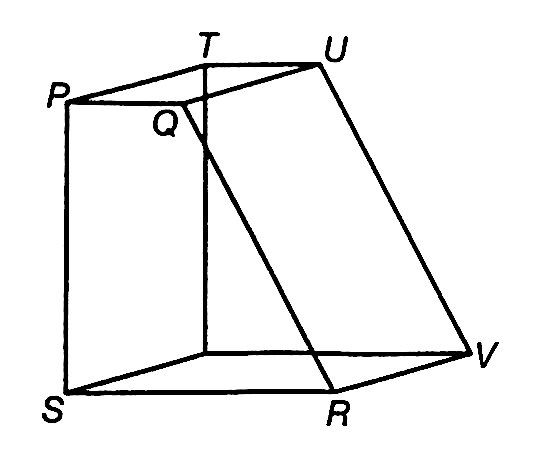
\includegraphics[width=0.25\textwidth]{./images/k2q5.jpeg}
                  \end{center}
                  Given that $PQ$ is $x\textit{cm}$, $PQ:PS:SR = 2:5:3$ and the area of its
                  cross-section is $A\textit{cm}^2$.
                  \begin{enumerate}
                        \item Express $A$ in terms of $x$. \sol{}
                              \begin{flalign*}
                                    PQ:PS         & = 2:5                                              \\
                                    \frac{PQ}{PS} & = \frac{2}{5}                                      \\
                                    \frac{x}{PS}  & = \frac{2}{5}                                      \\
                                    2PS           & = 5x                                               \\
                                    PS            & = \frac{5x}{2}                                     \\
                                    PQ:SR         & = 2:3                                              \\
                                    \frac{PQ}{SR} & = \frac{2}{3}                                      \\
                                    \frac{x}{SR}  & = \frac{2}{3}                                      \\
                                    2SR           & = 3x                                               \\
                                    SR            & = \frac{3x}{2}                                     \\
                                    A             & = \frac{1}{2}(PQ + SR) \cdot PS                    \\
                                                  & = \frac{1}{2}(x + \frac{3x}{2}) \cdot \frac{5x}{2} \\
                                                  & = \frac{25x^2}{8}   \eos
                              \end{flalign*}

                        \item \begin{enumerate}
                                    \item When the metal is heated, $x$ increases at the rate of
                                          $0.02\textit{cm}\textit{s}^{-1}$. Find the rate of change of the area, in
                                          $\textit{cm}^2\textit{s}^{-1}$, of the cross-section when $x = 4\textit{cm}$.
                                          \sol{}
                                          \begin{flalign*}
                                                \frac{dx}{dt} & = 0.02                             \\
                                                \frac{dA}{dx} & = \frac{25x}{4}                    \\
                                                \frac{dA}{dt} & = \frac{dA}{dx}\cdot \frac{dx}{dt} \\
                                                              & = \frac{25x}{4}\cdot \frac{2}{100} \\
                                                              & = \frac{1x}{8}
                                          \end{flalign*}
                                          When $x = 4\textit{cm}$, $\dfrac{dA}{dt} \frac{4}{8} = 0.5\textit{cm}^2\textit{s}^{-1}$. $\eos$

                                    \item Given the thickness of the metal is $\dfrac{2}{5}x\textit{cm}$, find the
                                          approximate change of the volume, in $\textit{cm}^3$, of the metal when $x$
                                          changes from $4\textit{cm}$ to $4.05\textit{cm}$. \sol{}
                                          \begin{flalign*}
                                                V             & = A \cdot \frac{2}{5}x               \\
                                                              & = \frac{25x^2}{8} \cdot \frac{2}{5}x \\
                                                              & = \frac{5x^3}{4}                     \\
                                                \frac{dV}{dx} & = \frac{15x^2}{4}
                                          \end{flalign*}
                                          When $x = 4\textit{cm}$,
                                          \begin{flalign*}
                                                V                         & = \dfrac{5{(4)}^3}{4} = 80           \\
                                                \frac{dV}{dx}             & = \dfrac{15{(4)}^2}{4} = 60          \\
                                                \frac{\delta V}{\delta x} & \approx \dfrac{dV}{dx}               \\
                                                \delta V                  & \approx \dfrac{dV}{dx}\cdot \delta x \\
                                                                          & = 60 \cdot (4.05 - 4)                \\
                                                                          & = 60 \cdot 0.05                      \\
                                                                          & = 3\textit{cm}^3 \eos
                                          \end{flalign*}
                              \end{enumerate}
                  \end{enumerate}

            \item A wire of length of $26\textit{cm}$ is bent to form a sector with centre $O$
                  and radius $r\textit{cm}$ as in the diagram below.
                  \begin{center}
                        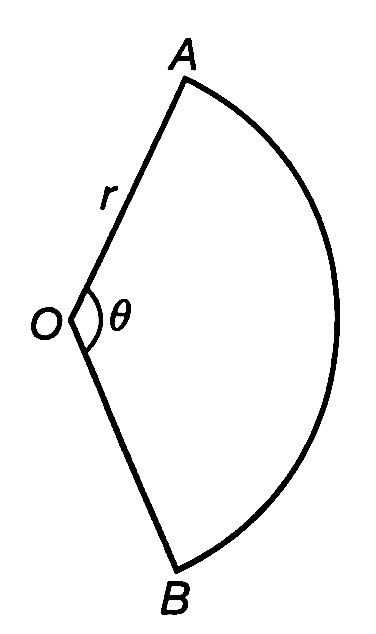
\includegraphics[width=0.15\textwidth]{./images/k2q6.jpeg}
                  \end{center}
                  \begin{enumerate}
                        \item Express $\theta$ in terms of $r$. \sol{}
                              \begin{flalign*}
                                    C       & = 2r + r\theta            \\
                                    26      & = 2r + r\theta            \\
                                    r\theta & = 26 - 2r                 \\
                                    \theta  & = \dfrac{26 - 2r}{r} \eos
                              \end{flalign*}

                        \item If the radius increases at the rate of $0.1\textit{cm}\textit{s}^{-1}$, find,
                              at the instant $r = 2\textit{cm}$,
                              \begin{enumerate}
                                    \item the rate of change, in $\textit{rad}\textit{s}^{-1}$, of $\theta$. \sol{}
                                          \begin{flalign*}
                                                \frac{dr}{dt}      & = 0.1                                   \\
                                                \frac{d\theta}{dr} & = \frac{1}{r}                           \\
                                                \frac{d\theta}{dr} & = -\frac{26}{r^2}                       \\
                                                \frac{d\theta}{dt} & = \frac{d\theta}{dr}\cdot \frac{dr}{dt} \\
                                                                   & = -\frac{26}{r^2}\cdot \frac{1}{10}     \\
                                                                   & = -\frac{13}{5r^2}                      \\
                                                                   & = -\frac{13}{5(2)^2}                    \\
                                                                   & = -\frac{13}{20}                        \\
                                                                   & = -0.65\textit{rad}\textit{s}^{-1} \eos
                                          \end{flalign*}

                                    \item the rate of change of the area, in $\textit{cm}^2\textit{s}^{-1}$, of the
                                          sector. \sol{}
                                          \begin{flalign*}
                                                A             & = \frac{1}{2}r^2\left(\frac{26-2r}{r}\right) \\
                                                              & = r(13-r)                                    \\
                                                              & = 13r - r^2                                  \\
                                                \frac{dA}{dr} & = 13 - 2r                                    \\
                                                \frac{dA}{dt} & = \frac{dA}{dr} \cdot \frac{dr}{dt}          \\
                                                              & = \frac{13 - 2r}{10}                         \\
                                                              & = \frac{13 - 2(2)}{10}                       \\
                                                              & = \frac{9}{10}                               \\
                                                              & = 0.9\textit{cm}^2\textit{s}^{-1} \eos
                                          \end{flalign*}
                              \end{enumerate}
                  \end{enumerate}

            \item A factory needs to produce containers of the same size for a type of breakfast
                  cereals as shown in the diagram below. Each container must have a volume of
                  $2666\dfrac{2}{3}\textit{cm}^3$. The base of the containers is rectangular in
                  shape with its length twice the width. In order to reduce the production cost,
                  the total surface area of each container must be minimum.
                  \begin{center}
                        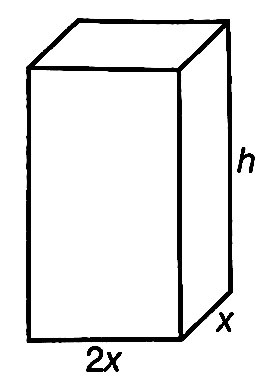
\includegraphics[width=0.15\textwidth]{./images/k2q7.jpeg}
                  \end{center}

                  \begin{enumerate}
                        \item Find the dimensions of the containers produced. \sol{}
                              \begin{flalign*}
                                    V     & = 2x \cdot x \cdot h                       \\
                                    2x^2h & = 2666\dfrac{2}{3}                         \\
                                          & = \dfrac{8000}{3}                          \\
                                    6x^2h & = 8000                                     \\
                                    h     & = \dfrac{4000}{3x^2} \eos                  \\
                                    A     & = 2(2xh) + 2(xh) + 2(2x^2)                 \\
                                          & = 4xh + 2xh + 4x^2                         \\
                                          & = 6xh + 4x^2                               \\
                                          & = 6x\left(\dfrac{4000}{3x^2}\right) + 4x^2 \\
                                          & = \dfrac{8000}{x} + 4x^2
                              \end{flalign*}
                              $A$ is minimum when $\frac{dA}{dx} = 0$.
                              \begin{flalign*}
                                    \frac{dA}{dx}          & = 8x - \dfrac{8000}{x^2} \\
                                    8x - \dfrac{8000}{x^2} & = 0                      \\
                                    8x^3 - 8000            & = 0                      \\
                                    x^3 - 1000             & = 0                      \\
                                    x^3                    & = 1000                   \\
                                    x                      & = 10                     \\
                                    h                      & = \dfrac{4000}{3(10)^2}  \\
                                                           & = \dfrac{4000}{300}      \\
                                                           & = \dfrac{40}{3}          \\
                                                           & = 13\dfrac{1}{3}
                              \end{flalign*}
                              Hence, the dimensions of the containers produced are $20\textit{cm} \times 10\textit{cm} \times 13\dfrac{1}{3}\textit{cm}$. $\eos$

                        \item Hence, find the total cost of production for $20000$ units of containers if the
                              cost of production for a containers is RM$0.002$ per $\textit{cm}^2$. \sol{}
                              \begin{flalign*}
                                    A & = \dfrac{8000}{x} + 4x^2       \\
                                      & = \dfrac{8000}{10} + 4{(10)}^2 \\
                                      & = 800 + 400                    \\
                                      & = 1200 \textit{cm}^2
                              \end{flalign*}
                              \begin{flalign*}
                                    \text{Cost per container}       & = 0.002 \times 1200    \\
                                                                    & = \text{RM}2.40        \\
                                    \text{Total cost of production} & = 20000 \times 2.40    \\
                                                                    & = \text{RM}48,000 \eos
                              \end{flalign*}
                  \end{enumerate}

            \item An opened right circular cone with the base radius $r\textit{cm}$ and slant
                  height $12\textit{cm}$ is used to cover a ball with radius $j\textit{cm}$ such
                  that the ball is inscribed in the cone as shown in the cross-section diagram
                  below.
                  \begin{center}
                        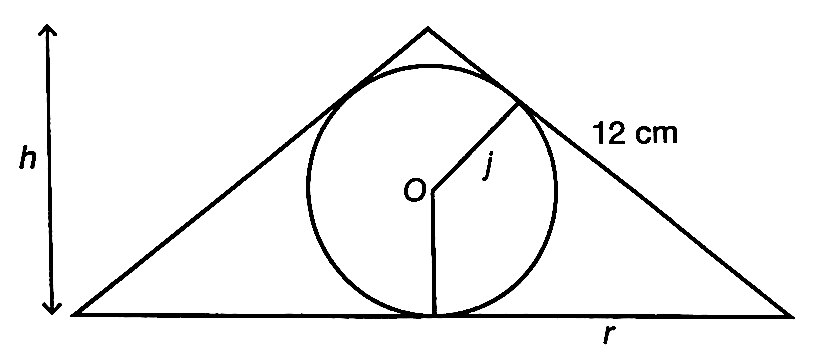
\includegraphics[width=0.35\textwidth]{./images/k2q8.jpeg}
                  \end{center}
                  Show that the volume of the cone is given by $V = \dfrac{\pi}{3}(144h - h^3)$.
                  Hence, determine the dimensions of the right circular cone such that its volume
                  is maximum and find the radius of the ball, $j$, which corresponded to the
                  maximum volume of the cone.
                  \sol{}
                  \begin{flalign*}
                        \sqrt{r^2 + h^2}  & = 144                             \\
                        r^2               & = 144 - h^2                       \\
                        V_{\textit{cone}} & = \dfrac{\pi}{3} r^2h             \\
                                          & = \dfrac{\pi}{3} (144 - h^2)h     \\
                                          & = \dfrac{\pi}{3} (144h - h^3)\eos
                  \end{flalign*}
                  $V_{\textit{cone}}$ is maximum when $\frac{dV_{\textit{cone}}}{dh} = 0$.
                  \begin{flalign*}
                        \frac{dV_{\textit{cone}}}{dh} & = \dfrac{\pi}{3}(144 - 3h^2)   \\
                        \dfrac{\pi}{3}(144 - 3h^2)    & = 0                            \\
                        144 - 3h^2                    & = 0                            \\
                        h^2                           & = 48                           \\
                        h                             & = 4\sqrt{3} \quad (h > 0) \eos \\
                        r                             & = \sqrt{144 - {(4\sqrt{3})}^2} \\
                                                      & = 4\sqrt{6} \eos               \\
                        \\
                        \sin {2\alpha}                & = \frac{4\sqrt{3}}{12}         \\
                                                      & = \frac{\sqrt{3}}{3}           \\
                                                      & = 35.2644^{\circ}              \\
                        \alpha                        & = 17.6322^{\circ}              \\
                        \tan 17.6322                  & = \frac{j}{4\sqrt{6}}          \\
                        j                             & = 4\sqrt{6}\tan 17.6322        \\
                                                      & = 3.1142\textit{cm} \eos
                  \end{flalign*}

      \end{enumerate}
\end{multicols*}

\end{document}